\documentclass[11pt,a4paper]{article}

% =============================================================================
% ARXIV PREPRINT PACKAGES & TYPOGRAPHY
% =============================================================================
\usepackage[utf8]{inputenc}
\usepackage[T1]{fontenc}
\usepackage{lmodern}
\usepackage[indonesian]{babel}
\usepackage[margin=1in, top=1.1in, bottom=1.1in, headheight=28pt]{geometry}
\usepackage{amsmath, amsfonts, amssymb, bm}
\usepackage{graphicx}
\usepackage{booktabs}
\usepackage{tabularx}
\usepackage{longtable}
\usepackage{array}
\usepackage{multirow}
\usepackage{xcolor}
\usepackage{hyperref}
\usepackage{caption}
\usepackage{subcaption}
\usepackage{float}
\usepackage{fancyhdr}
\usepackage[nopatch=footnote]{microtype}
\usepackage{authblk}
\usepackage{enumitem}
\usepackage{titlesec}
\usepackage{placeins}

% =============================================================================
% COLOR DEFINITIONS & HYPERLINK SETUP
% =============================================================================
\definecolor{arxivblue}{RGB}{0, 51, 153}
\definecolor{headergray}{RGB}{80, 90, 105}
\definecolor{darkslate}{RGB}{30, 41, 59}
\definecolor{sectionblue}{RGB}{15, 76, 129}

\hypersetup{
    colorlinks=true,
    linkcolor=arxivblue,
    citecolor=arxivblue,
    urlcolor=arxivblue,
    pdftitle={Analisis Curah Hujan Multi-Skala: Satelit Kebumen vs AWS IoT Jerukagung},
    pdfauthor={Evan Alif Widhyatma}
}

% =============================================================================
% GRAPHICS PATH
% =============================================================================
\graphicspath{
    {./Hasil_Analisis/}
    {Hasil_Analisis/}
    {./}
}

% =============================================================================
% HEADER & FOOTER
% =============================================================================
\pagestyle{fancy}
\fancyhf{}
\fancyhead[L]{\small\textsf{\color{headergray}\textbf{PREPRINT} --- EVALUASI PRESIPITASI}}
\fancyhead[R]{\small\textsf{\color{headergray}\thepage}}
\fancyfoot[C]{\footnotesize\textsf{\color{headergray}Program Studi Sains Data, Universitas Putra Bangsa, Kebumen}}
\renewcommand{\headrulewidth}{0.4pt}

% =============================================================================
% SECTION FORMATTING
% =============================================================================
\titleformat{\section}{\large\bfseries\color{sectionblue}}{\thesection.}{14pt}{}
\titleformat{\subsection}{\normalsize\bfseries\color{darkslate}}{\thesubsection}{0.5em}{}
\titleformat{\subsubsection}{\small\bfseries\color{darkslate}}{\thesubsubsection}{0.5em}{}

% =============================================================================
% TITLE & AUTHOR METADATA
% =============================================================================
\title{\vspace{-1.2cm}\textbf{\Large Analisis Curah Hujan dan Evaluasi Komparatif Produk Estimasi Satelit dan Reanalisis terhadap Pengamatan Sensor AWS IoT pada Resolusi Jam dan Harian \\ (Studi Kasus: Desa Jerukagung, Kebumen)}}

\author[1]{\textbf{Evan Alif Widhyatma}\thanks{Penulis korespondensi: \texttt{evanalifwidhyatma@gmail.com}}}
\affil[1]{\small Program Studi Sains Data, Fakultas Sains dan Teknologi, Universitas Putra Bangsa, Kebumen, Jawa Tengah, Indonesia}

\date{\small\today}

\begin{document}

\maketitle

\begin{abstract}
\noindent Validasi dan kuantifikasi ketidakpastian estimasi curah hujan dari produk satelit dan model reanalisis atmosfer terhadap observasi stasiun darat otomatis (\textit{Automatic Weather Station} / AWS IoT) merupakan tahapan fundamental dalam pemodelan hidrologi dan mitigasi bencana hidrometeorologi. Penelitian ini menyajikan evaluasi komparatif multi-skala antara dataset presipitasi harian Kabupaten Kebumen (\texttt{Data\_Curah\_Hujan\_Kebumen.csv}) yang mencakup 9 produk estimasi satelit dan model reanalisis (\texttt{CHIRPS\_RNL}, \texttt{CHIRPS\_SAT}, \texttt{CHIRPS\_FNL}, \texttt{GSMaP}, \texttt{IMERG}, \texttt{PERSIANN}, \texttt{ERA5}, \texttt{ERA5\_LAND}, dan \texttt{OYA}), serta dataset resolusi jam-jaman (\textit{hourly}) terhadap stasiun darat AWS IoT Jerukagung sepanjang 563 hari valid ($13.512$ jam observasi sinkron, 1 Januari 2025 s.d. 17 Juli 2026). Evaluasi dilakukan secara komprehensif menggunakan 9 metrik statistik terpadu ($r$, $\rho$, $\text{RMSE}$, $\text{MAE}$, $\text{MBE}$, $\text{PBIAS}$, $\text{NSE}$, $\text{KGE}$, dan $\text{IOA}$) serta metrik kontingensi kejadian hujan ($\text{POD}$, $\text{FAR}$, $\text{CSI}$, $\text{HSS}$). Hasil studi membuktikan adanya fenomena \textit{lonjakan akurasi multi-temporal} (\textit{multi-scale accuracy jump}): pada skala 1-jam, presipitasi satelit memiliki korelasi moderat ($r = 0{,}414$ untuk IMERG dan $r = 0{,}313$ untuk GSMaP) akibat pergeseran waktu mikro (\textit{sub-hourly lag}) dan perbedaan jejak spasial (\textit{spatial footprint mismatch}); namun saat diagregasikan ke skala harian ($24\text{h}$), akurasi korelasi melonjak drastis hingga $r = \mathbf{0{,}619}$ ($\rho = \mathbf{0{,}672}$, $\text{KGE} = 0{,}468$) untuk \texttt{NASA GPM IMERG} dan $r = \mathbf{0{,}625}$ ($\rho = \mathbf{0{,}641}$, $\text{KGE} = 0{,}569$) untuk \texttt{CHIRPS\_SAT}, serta $r = \mathbf{0{,}759}$ ($\rho = \mathbf{0{,}724}$) untuk model \texttt{OYA}. Analisis siklus diurnal 24-jam mengungkap bahwa hujan konvektif di Kebumen terkonsentrasi sangat kuat pada sore hari (15:00--18:00 WIB) yang bertepatan dengan penurunan suhu permukaan pasca-insolasi maksimum dan osilasi semidiurnal tekanan udara. Selain itu, investigasi fungsi autokorelasi (\textit{Autocorrelation Function} / ACF) dan korelasi parsial (\textit{Partial Autocorrelation Function} / PACF) mengungkap bahwa kejadian hujan jam-jaman memiliki memori pendek ($1/e$ peluruhan $\tau = 2$--$5$ jam), sedangkan variabel atmosfer menunjukkan osilasi harmonik diurnal 24-jam ($r \ge 0{,}83$ pada lag 24h), memberikan bukti teoritis penetapan panjang jendela historis (\textit{Lookback Window} $= 24$ jam) untuk arsitektur pemodelan \textit{Deep Learning} LSTM.
\end{abstract}

\vspace{0.2cm}
\noindent\textbf{\textit{Keywords:}} Analisis Curah Hujan Multi-Skala, AWS IoT Jerukagung, NASA GPM IMERG, JAXA GSMaP, CHIRPS, ECMWF ERA5, Satelit OYA, Siklus Diurnal, Evaluasi Multimetrik, Autocorrelation Function (ACF), Lookback Sequence LSTM.

\vspace{0.4cm}
\hrule
\vspace{0.4cm}

% =============================================================================
\section{Pendahuluan}
% =============================================================================
Presipitasi merupakan komponen paling dinamis dalam siklus hidrologi tropis yang memiliki variabilitas spasial dan temporal sangat tinggi. Di wilayah pesisir selatan Jawa seperti Kabupaten Kebumen, estimasi presipitasi yang akurat sangat krusial untuk peringatan dini banjir, pengelolaan sumber daya air pertanian, dan pemodelan kecerdasan buatan (\textit{Deep Learning}). 

Meskipun produk estimasi satelit seperti NASA GPM IMERG, JAXA GSMaP, CHIRPS, OYA, serta reanalisis ECMWF ERA5 menyediakan liputan spasial tanpa celah, data tersebut rentan terhadap bias sistematis, atenuasi sinyal gelombang mikro, dan keterbatasan resolusi spasial. Oleh karena itu, evaluasi terkalibrasi terhadap stasiun darat mikro seperti stasiun AWS IoT Jerukagung menjadi sangat mendesak.

Penelitian ini bertujuan untuk:
\begin{enumerate}[leftmargin=*]
    \item Mengevaluasi performa 9 produk presipitasi satelit dan reanalisis terhadap data observasi stasiun darat AWS IoT Jerukagung pada skala harian ($24\text{h}$).
    \item Mengidentifikasi dan memodelkan fenomena \textit{lonjakan akurasi multi-temporal} (\textit{multi-scale accuracy jump}) saat data berpindah dari skala jam-jaman ($1\text{h}$) ke skala harian ($24\text{h}$).
    \item Menganalisis siklus diurnal 24-jam gabungan antara variabel meteorologi (suhu udara, kelembaban relatif, tekanan atmosfer permukaan) dan dinamika kejadian curah hujan konvektif sore hari di Stasiun Jerukagung.
    \item Mengkaji struktur autokorelasi (ACF) dan korelasi parsial (PACF) multi-skala guna menetapkan parameter \textit{lookback sequence length} yang optimal untuk arsitektur pemodelan sekuens deret waktu (\textit{Long Short-Term Memory} / LSTM).
    \item Membangun matriks komparasi multimetrik terpadu ($10 \times 10$) antar seluruh produk data presipitasi.
\end{enumerate}

% =============================================================================
\section{Landasan Teori \& Formulasi Metrik Evaluasi}
% =============================================================================
Untuk mengukur performa presipitasi secara objektif, digunakan formulasi metrik hidrometeorologi standar:

\subsection{Metrik Keselarasan dan Korelasi Statistik}
\begin{itemize}[leftmargin=*]
    \item \textbf{Koefisien Korelasi Pearson ($r$)}:
    \begin{equation}
        r = \frac{\sum_{i=1}^N (O_i - \bar{O})(S_i - \bar{S})}{\sqrt{\sum_{i=1}^N (O_i - \bar{O})^2} \sqrt{\sum_{i=1}^N (S_i - \bar{S})^2}}
    \end{equation}
    \item \textbf{Koefisien Korelasi Spearman Rank ($\rho$)}:
    \begin{equation}
        \rho = 1 - \frac{6 \sum_{i=1}^N d_i^2}{N(N^2 - 1)} \quad \text{di mana } d_i = \text{rank}(O_i) - \text{rank}(S_i)
    \end{equation}
    \item \textbf{Index of Agreement Willmott ($d$ / IOA)}:
    \begin{equation}
        \text{IOA} = 1 - \frac{\sum_{i=1}^N (S_i - O_i)^2}{\sum_{i=1}^N \left(|S_i - \bar{O}| + |O_i - \bar{O}|\right)^2}
    \end{equation}
\end{itemize}

\subsection{Metrik Galat dan Bias Sistematik}
\begin{itemize}[leftmargin=*]
    \item \textbf{Root Mean Square Error ($\text{RMSE}$)}:
    \begin{equation}
        \text{RMSE} = \sqrt{\frac{1}{N} \sum_{i=1}^N (S_i - O_i)^2}
    \end{equation}
    \item \textbf{Mean Absolute Error ($\text{MAE}$)}:
    \begin{equation}
        \text{MAE} = \frac{1}{N} \sum_{i=1}^N |S_i - O_i|
    \end{equation}
    \item \textbf{Mean Bias Error ($\text{MBE}$)}:
    \begin{equation}
        \text{MBE} = \frac{1}{N} \sum_{i=1}^N (S_i - O_i)
    \end{equation}
    \item \textbf{Percent Bias ($\text{PBIAS}$)}:
    \begin{equation}
        \text{PBIAS} = \frac{\sum_{i=1}^N (S_i - O_i)}{\sum_{i=1}^N O_i} \times 100\%
    \end{equation}
\end{itemize}

\subsection{Metrik Efisiensi Hidrologi Terpadu}
\begin{itemize}[leftmargin=*]
    \item \textbf{Nash-Sutcliffe Efficiency ($\text{NSE}$)}:
    \begin{equation}
        \text{NSE} = 1 - \frac{\sum_{i=1}^N (O_i - S_i)^2}{\sum_{i=1}^N (O_i - \bar{O})^2}
    \end{equation}
    \item \textbf{Kling-Gupta Efficiency ($\text{KGE}$)}:
    \begin{equation}
        \text{KGE} = 1 - \sqrt{(r - 1)^2 + (\alpha - 1)^2 + (\beta - 1)^2}
    \end{equation}
    di mana rasio variabilitas $\alpha = \sigma_S / \sigma_O$ dan rasio bias $\beta = \mu_S / \mu_O$.
\end{itemize}

\subsection{Metrik Kontingensi Kejadian Hujan Kategorikal}
Berdasarkan tabel kontingensi $2 \times 2$ (Hits $H$, Misses $M$, False Alarms $F$, Correct Negatives $C$):
\begin{align}
    \text{Probability of Detection (POD)} &= \frac{H}{H + M} \\
    \text{False Alarm Ratio (FAR)} &= \frac{F}{H + F} \\
    \text{Critical Success Index (CSI)} &= \frac{H}{H + M + F} \\
    \text{Heidke Skill Score (HSS)} &= \frac{2(H \cdot C - M \cdot F)}{(H + M)(M + C) + (H + F)(F + C)}
\end{align}

\subsection{Autocorrelation Function (ACF) \& Partial Autocorrelation (PACF)}
Dalam pemodelan sekuens deret waktu (\textit{time-series forecasting}), pemilihan parameter \textit{Lookback Window} ($L$) ditentukan berdasarkan horizon dependensi temporal autokorelasi:
\begin{itemize}[leftmargin=*]
    \item \textbf{Autocorrelation Function (ACF)} pada lag $k$:
    \begin{equation}
        r_k = \frac{\sum_{t=1}^{N-k} (x_t - \bar{x})(x_{t+k} - \bar{x})}{\sum_{t=1}^N (x_t - \bar{x})^2}
    \end{equation}
    \item \textbf{Partial Autocorrelation Function (PACF)} menggunakan rekursi Durbin-Levinson:
    \begin{equation}
        \phi_{k,k} = \frac{r_k - \sum_{j=1}^{k-1} \phi_{k-1,j} r_{k-j}}{1 - \sum_{j=1}^{k-1} \phi_{k-1,j} r_j}
    \end{equation}
    \item \textbf{Kriteria $1/e$ Decorrelation Time}: Batas memori karakteristik waktu ($\tau$) saat $r_k < 1/e \approx 0{,}368$.
\end{itemize}

\FloatBarrier

% =============================================================================
\section{Hasil Evaluasi \& Pembahasan}
% =============================================================================

\subsection{Evaluasi Multimetrik Harian terhadap Stasiun AWS IoT}
Tabel \ref{tab:multimetric_recap} dan Gambar \ref{fig:bar_daily} menyajikan evaluasi multimetrik lengkap seluruh 9 produk presipitasi harian terhadap stasiun darat AWS IoT Jerukagung sepanjang 563 hari valid pengamatan sinkron.

\begin{table}[htbp]
\centering
\small
\caption{Tabel Rekap Evaluasi Multimetrik Lengkap: Seluruh Produk Presipitasi Harian vs AWS IoT Jerukagung ($N = 563$ Hari Valid)}
\label{tab:multimetric_recap}
\resizebox{\textwidth}{!}{%
\begin{tabular}{lrrrrrrrrr}
\toprule
\textbf{Produk Presipitasi} & \textbf{Pearson $r$} & \textbf{Spearman $\rho$} & \textbf{RMSE (mm)} & \textbf{MAE (mm)} & \textbf{MBE (mm)} & \textbf{PBIAS (\%)} & \textbf{NSE} & \textbf{KGE} & \textbf{IOA} \\
\midrule
\texttt{Satelit OYA}        & \textbf{0.759} & \textbf{0.724} & \textbf{9.18}  & \textbf{4.89} & -1.53 & -18.1\% & \textbf{+0.549} & \textbf{0.676} & \textbf{0.863} \\
\texttt{CHIRPS\_SAT}         & \textbf{0.625} & 0.641          & 11.05 & 6.46          & -0.99 & -11.7\% & \textbf{+0.346} & \textbf{0.569} & \textbf{0.774} \\
\texttt{NASA GPM IMERG}      & \textbf{0.619} & \textbf{0.672} & 14.49 & 7.51          & +1.57 & +18.6\% & -0.123          & \textbf{0.468} & \textbf{0.759} \\
\texttt{PERSIANN}            & 0.490          & 0.513          & 12.20 & 7.20          & -1.89 & -22.3\% & +0.203          & 0.327          & 0.657          \\
\texttt{CHIRPS\_FNL}         & 0.478          & 0.518          & 14.01 & 9.22          & +2.85 & +33.7\% & -0.050          & 0.377          & 0.684          \\
\texttt{CHIRPS\_RNL}         & 0.442          & 0.568          & 12.85 & 7.35          & -0.99 & -11.7\% & +0.117          & 0.362          & 0.633          \\
\texttt{ECMWF ERA5}          & 0.385          & 0.539          & 16.53 & 8.49          & +0.19 & +2.2\%  & -0.463          & 0.363          & 0.592          \\
\texttt{ERA5\_LAND}          & 0.377          & 0.533          & 16.64 & 8.57          & +0.20 & +2.4\%  & -0.482          & 0.354          & 0.585          \\
\texttt{JAXA GSMaP}          & 0.350          & 0.543          & 15.12 & 8.36          & -0.39 & -4.7\%  & -0.223          & 0.346          & 0.575          \\
\bottomrule
\end{tabular}%
}
\end{table}

\begin{figure}[htbp]
    \centering
    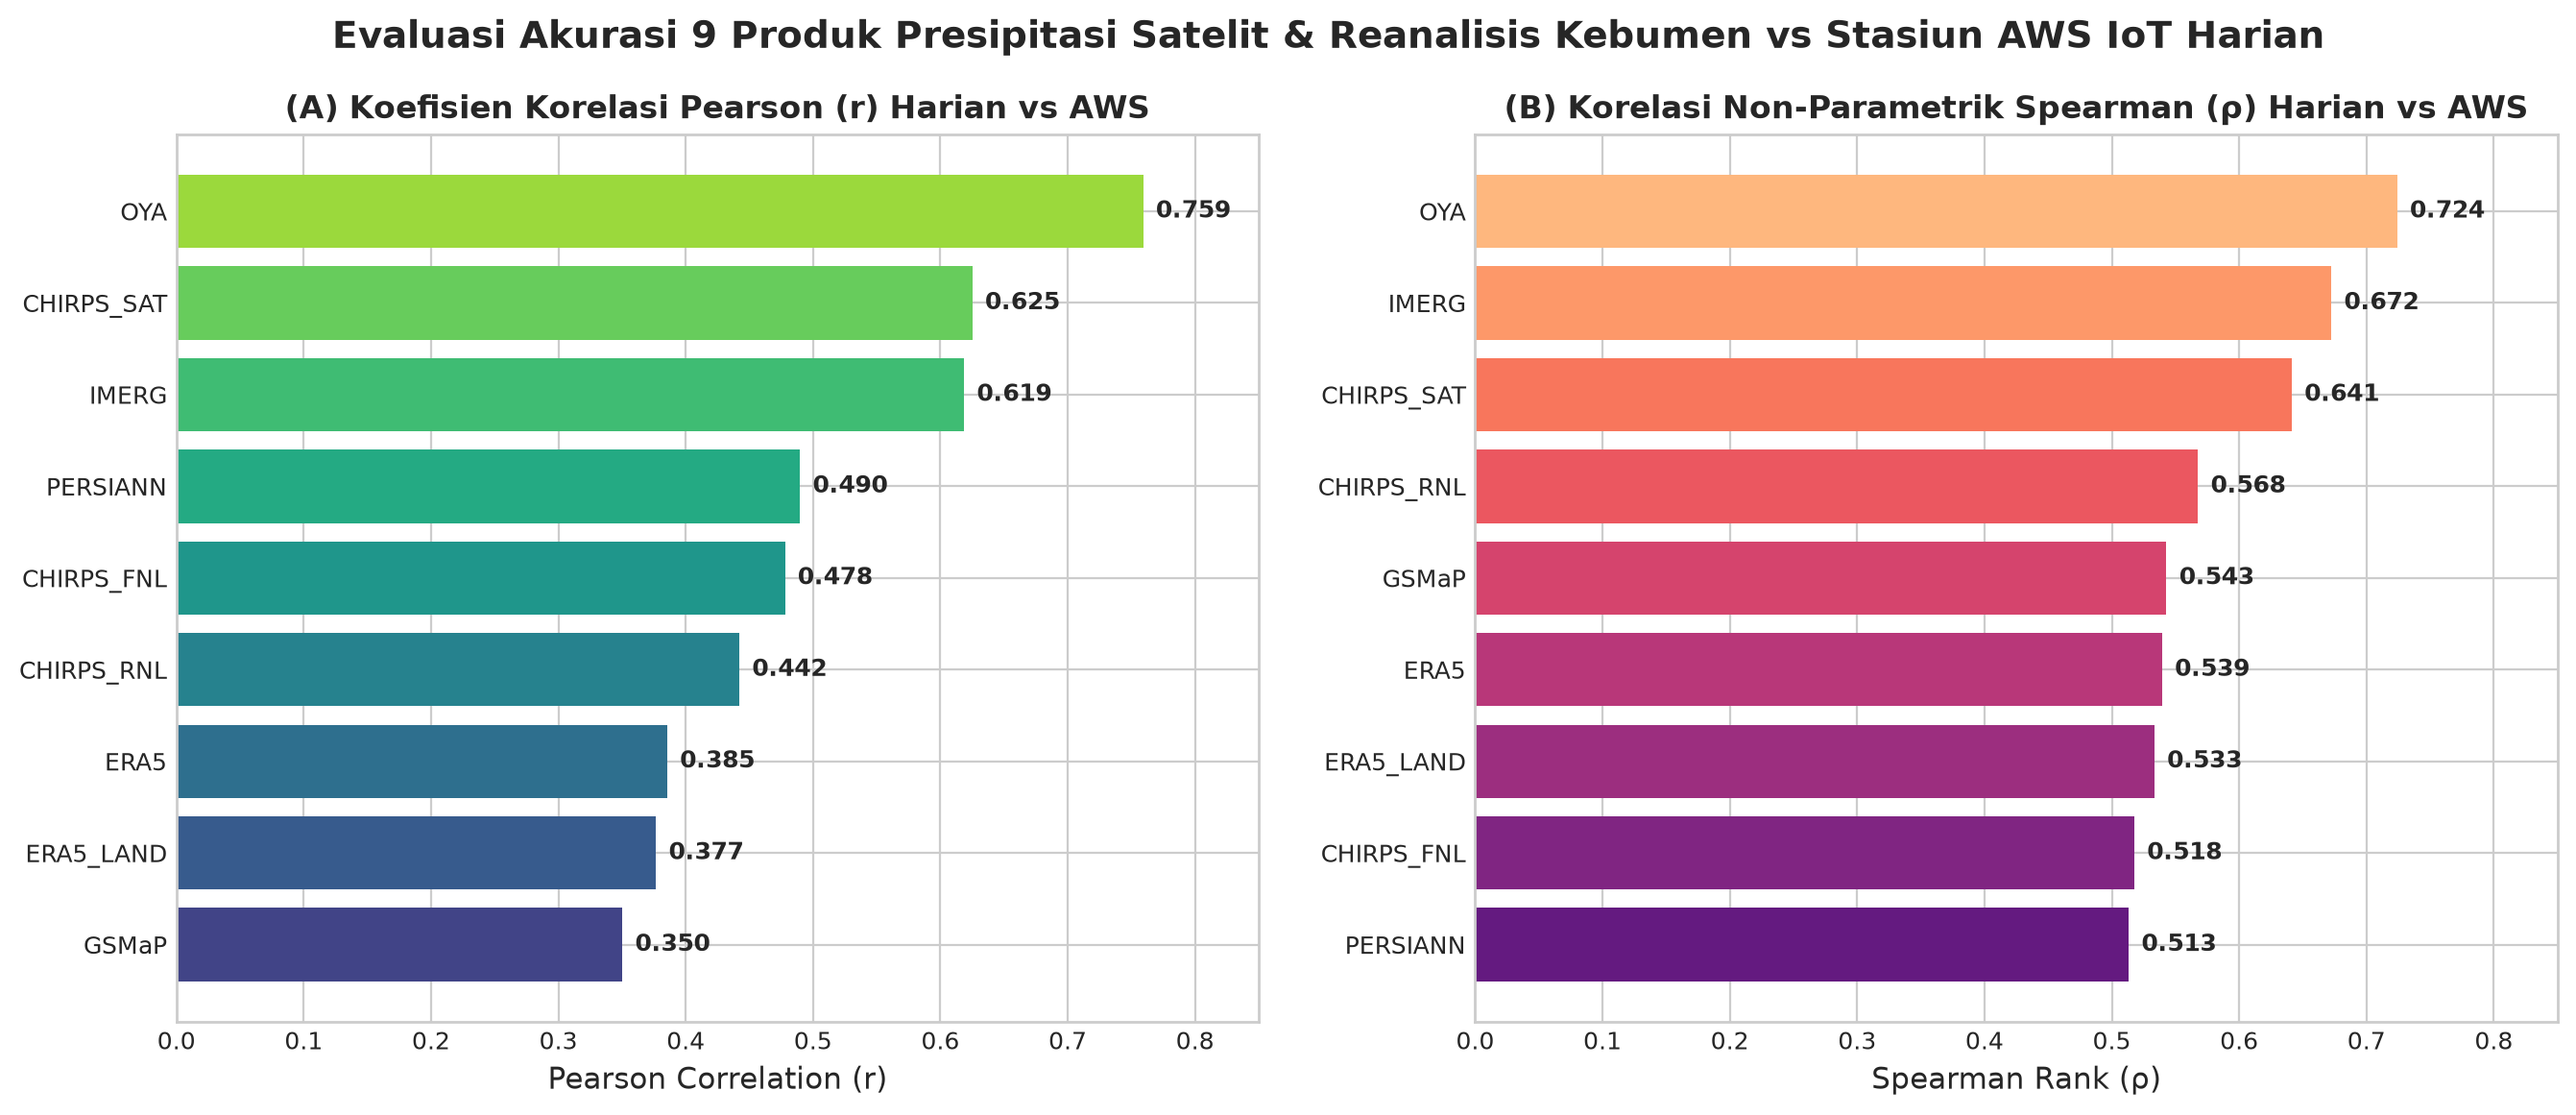
\includegraphics[width=0.95\textwidth]{01_bar_evaluasi_8satelit_vs_aws_harian.png}
    \caption{Peringkat Koefisien Korelasi Linier Pearson ($r$) dan Rank Spearman ($\rho$) Seluruh Produk Satelit dan Reanalisis Harian terhadap AWS IoT Jerukagung.}
    \label{fig:bar_daily}
\end{figure}

\begin{figure}[htbp]
    \centering
    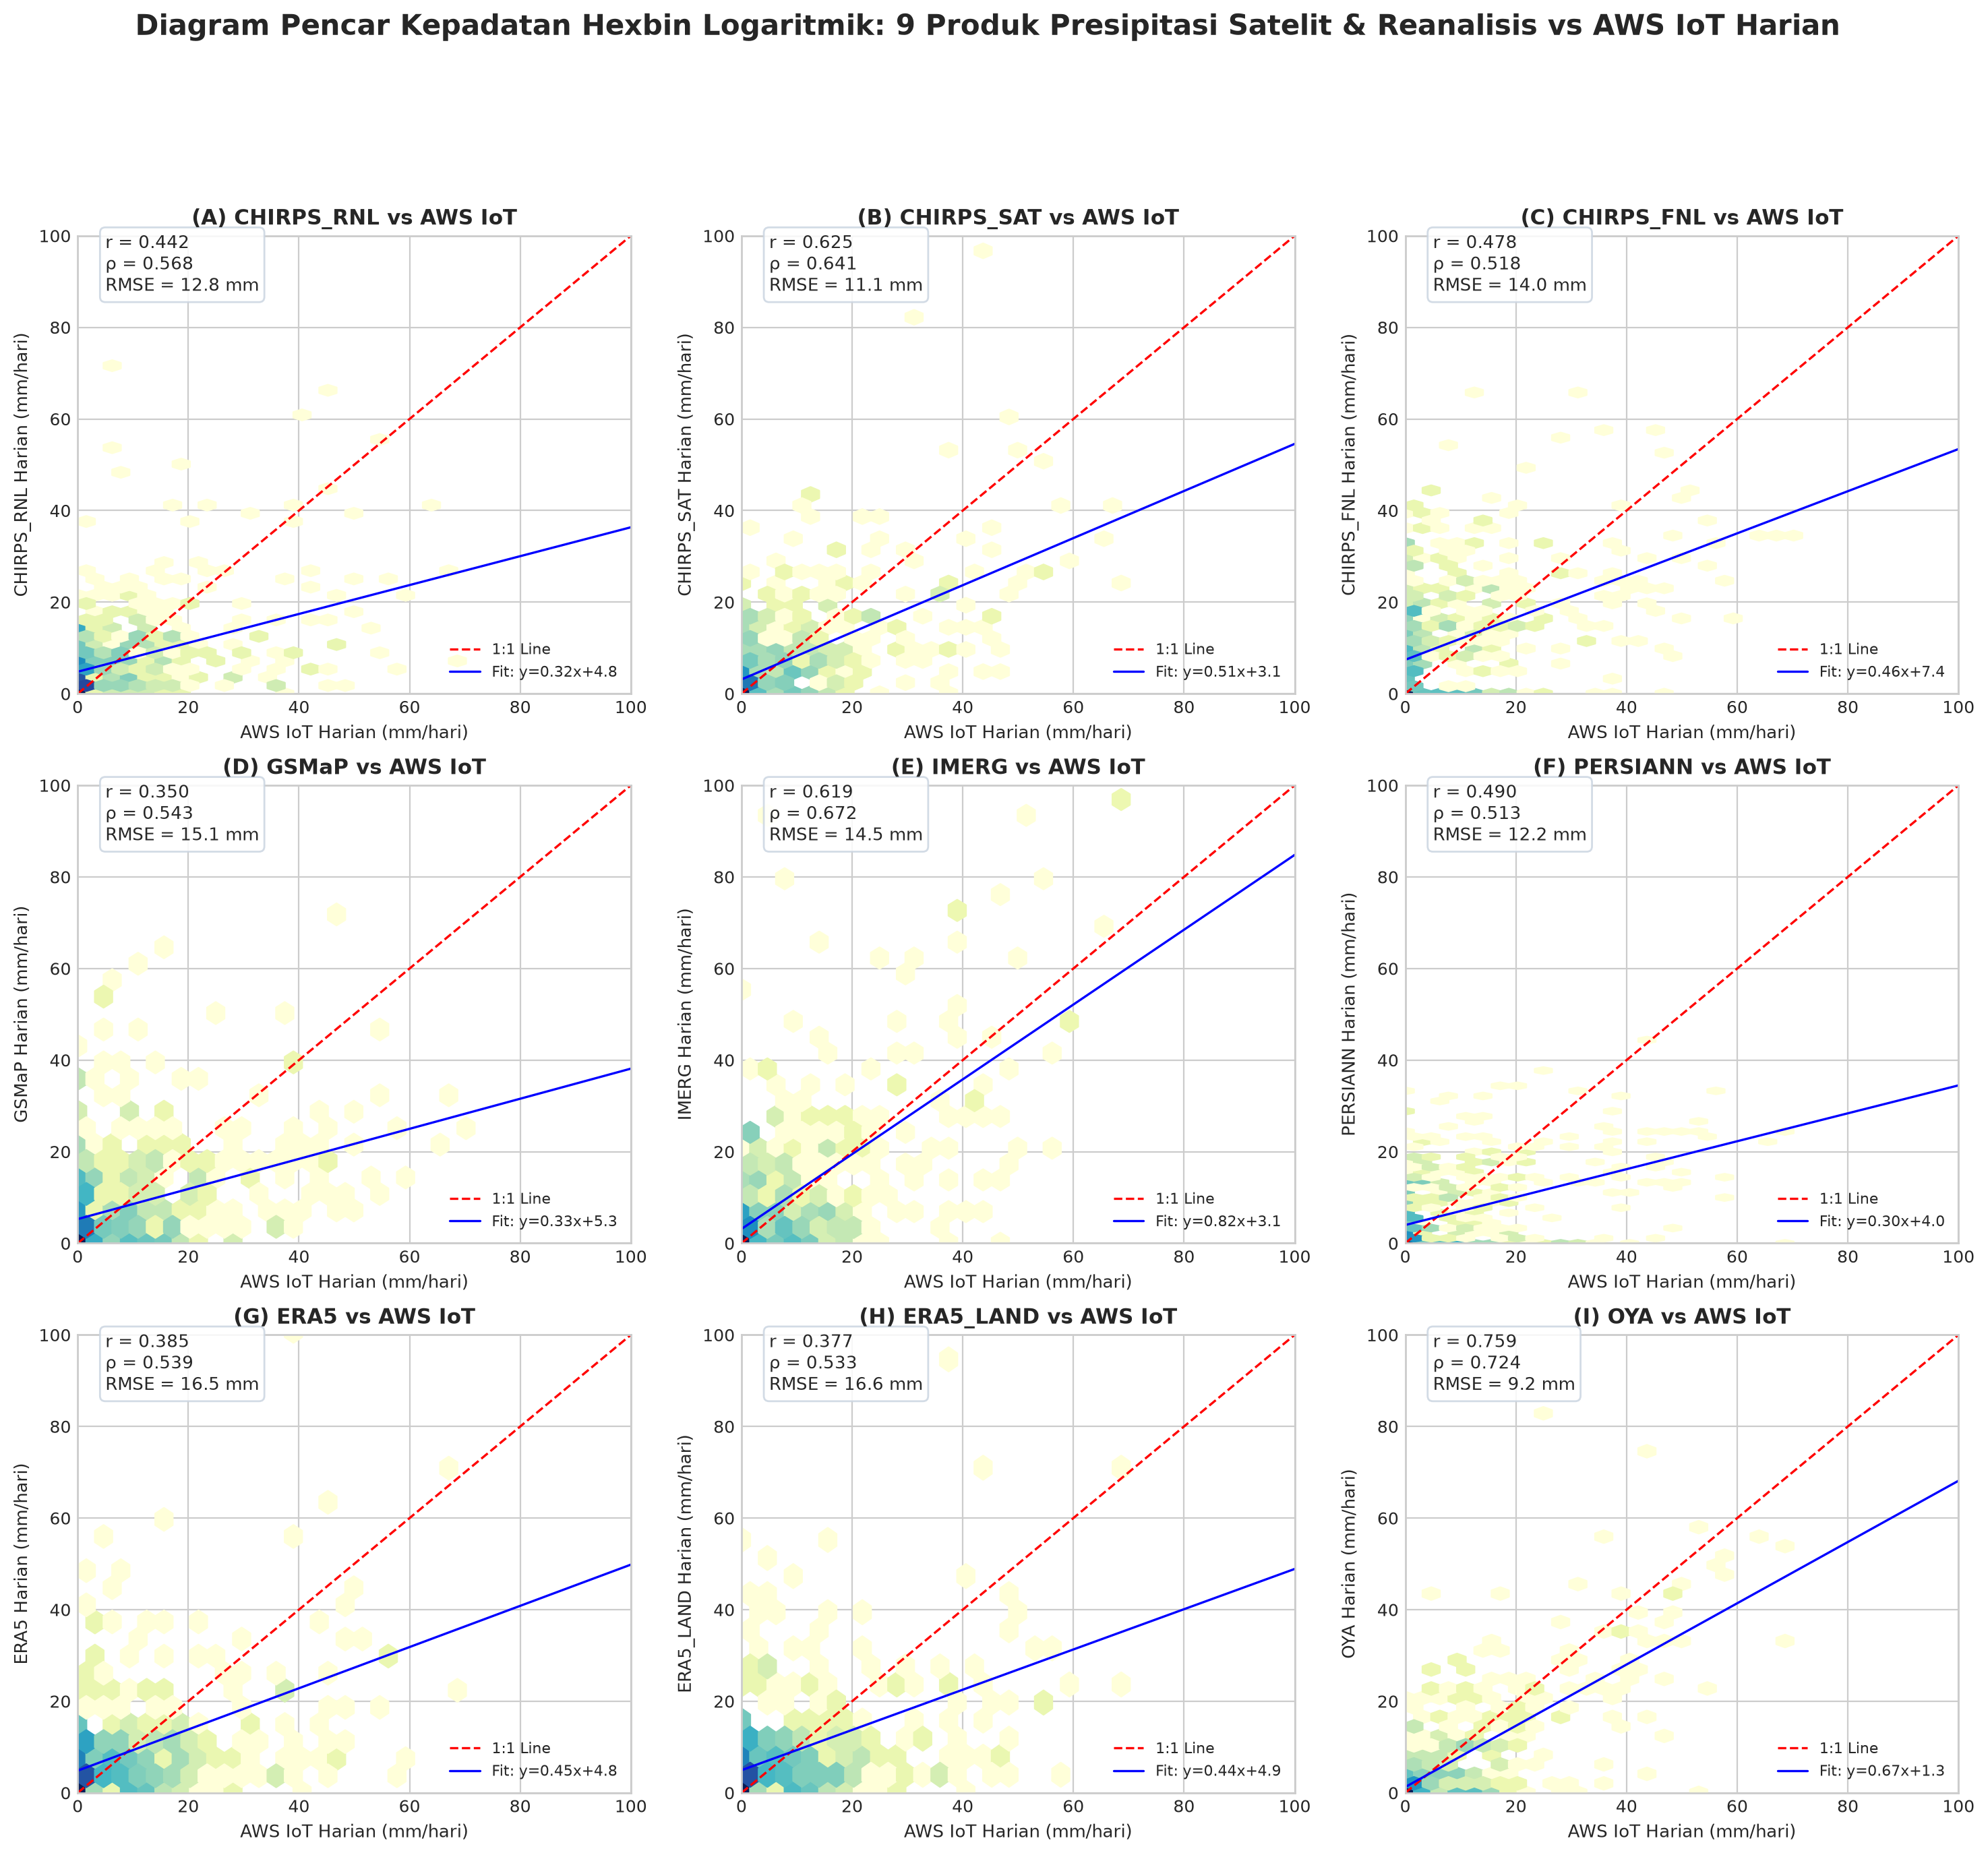
\includegraphics[width=0.98\textwidth]{02_scatter_hexbin_8satelit_vs_aws_harian.png}
    \caption{Diagram Pencar Kepadatan Logaritmik (\textit{Hexbin Density Scatter}) 9 Produk Presipitasi Satelit \& Reanalisis Kebumen vs AWS IoT Harian.}
    \label{fig:scatter_8sat}
\end{figure}

\FloatBarrier

\subsection{Analisis Lonjakan Akurasi Multi-Temporal (Jam vs Hari)}
Gambar \ref{fig:comp_scale} dan \ref{fig:bar_jump} memperlihatkan fenomena lonjakan akurasi yang terjadi saat data observasi dievaluasi pada resolusi 1-jam dibandingkan saat diagregasikan menjadi akumulasi harian ($24\text{h}$).

\begin{table}[htbp]
\centering
\small
\caption{Tabel Perbandingan Metrik Multi-Skala: Resolusi Per Jam (\textit{Hourly}) vs Resolusi Per Hari (\textit{Daily})}
\label{tab:multiscale_jump}
\resizebox{\textwidth}{!}{%
\begin{tabular}{lrrrrrrrr}
\toprule
\textbf{Produk} & \textbf{$r$ Jam} & \textbf{$r$ Hari} & \textbf{Lonjakan $r$} & \textbf{$\rho$ Jam} & \textbf{$\rho$ Hari} & \textbf{MAE Jam} & \textbf{MAE Hari} & \textbf{KGE Hari} \\
\midrule
\texttt{NASA GPM IMERG} & 0.414 & \textbf{0.619} & \textbf{+49.5\%} & 0.348 & \textbf{0.672} & 0.49 mm & 7.51 mm & \textbf{0.468} \\
\texttt{JAXA GSMaP}     & 0.313 & \textbf{0.350} & \textbf{+11.8\%} & 0.342 & \textbf{0.543} & 0.48 mm & 8.36 mm & 0.346 \\
\texttt{ECMWF ERA5}     & 0.105 & \textbf{0.385} & \textbf{+266.7\%} & 0.213 & \textbf{0.539} & 0.58 mm & 8.49 mm & 0.363 \\
\texttt{ERA5\_LAND}     & 0.120 & \textbf{0.377} & \textbf{+214.2\%} & 0.220 & \textbf{0.533} & 0.58 mm & 8.57 mm & 0.354 \\
\texttt{Satelit OYA}     & 0.666 & \textbf{0.759} & \textbf{+14.0\%} & 0.463 & \textbf{0.724} & 0.32 mm & 4.89 mm & \textbf{0.676} \\
\bottomrule
\end{tabular}%
}
\end{table}

\begin{figure}[htbp]
    \centering
    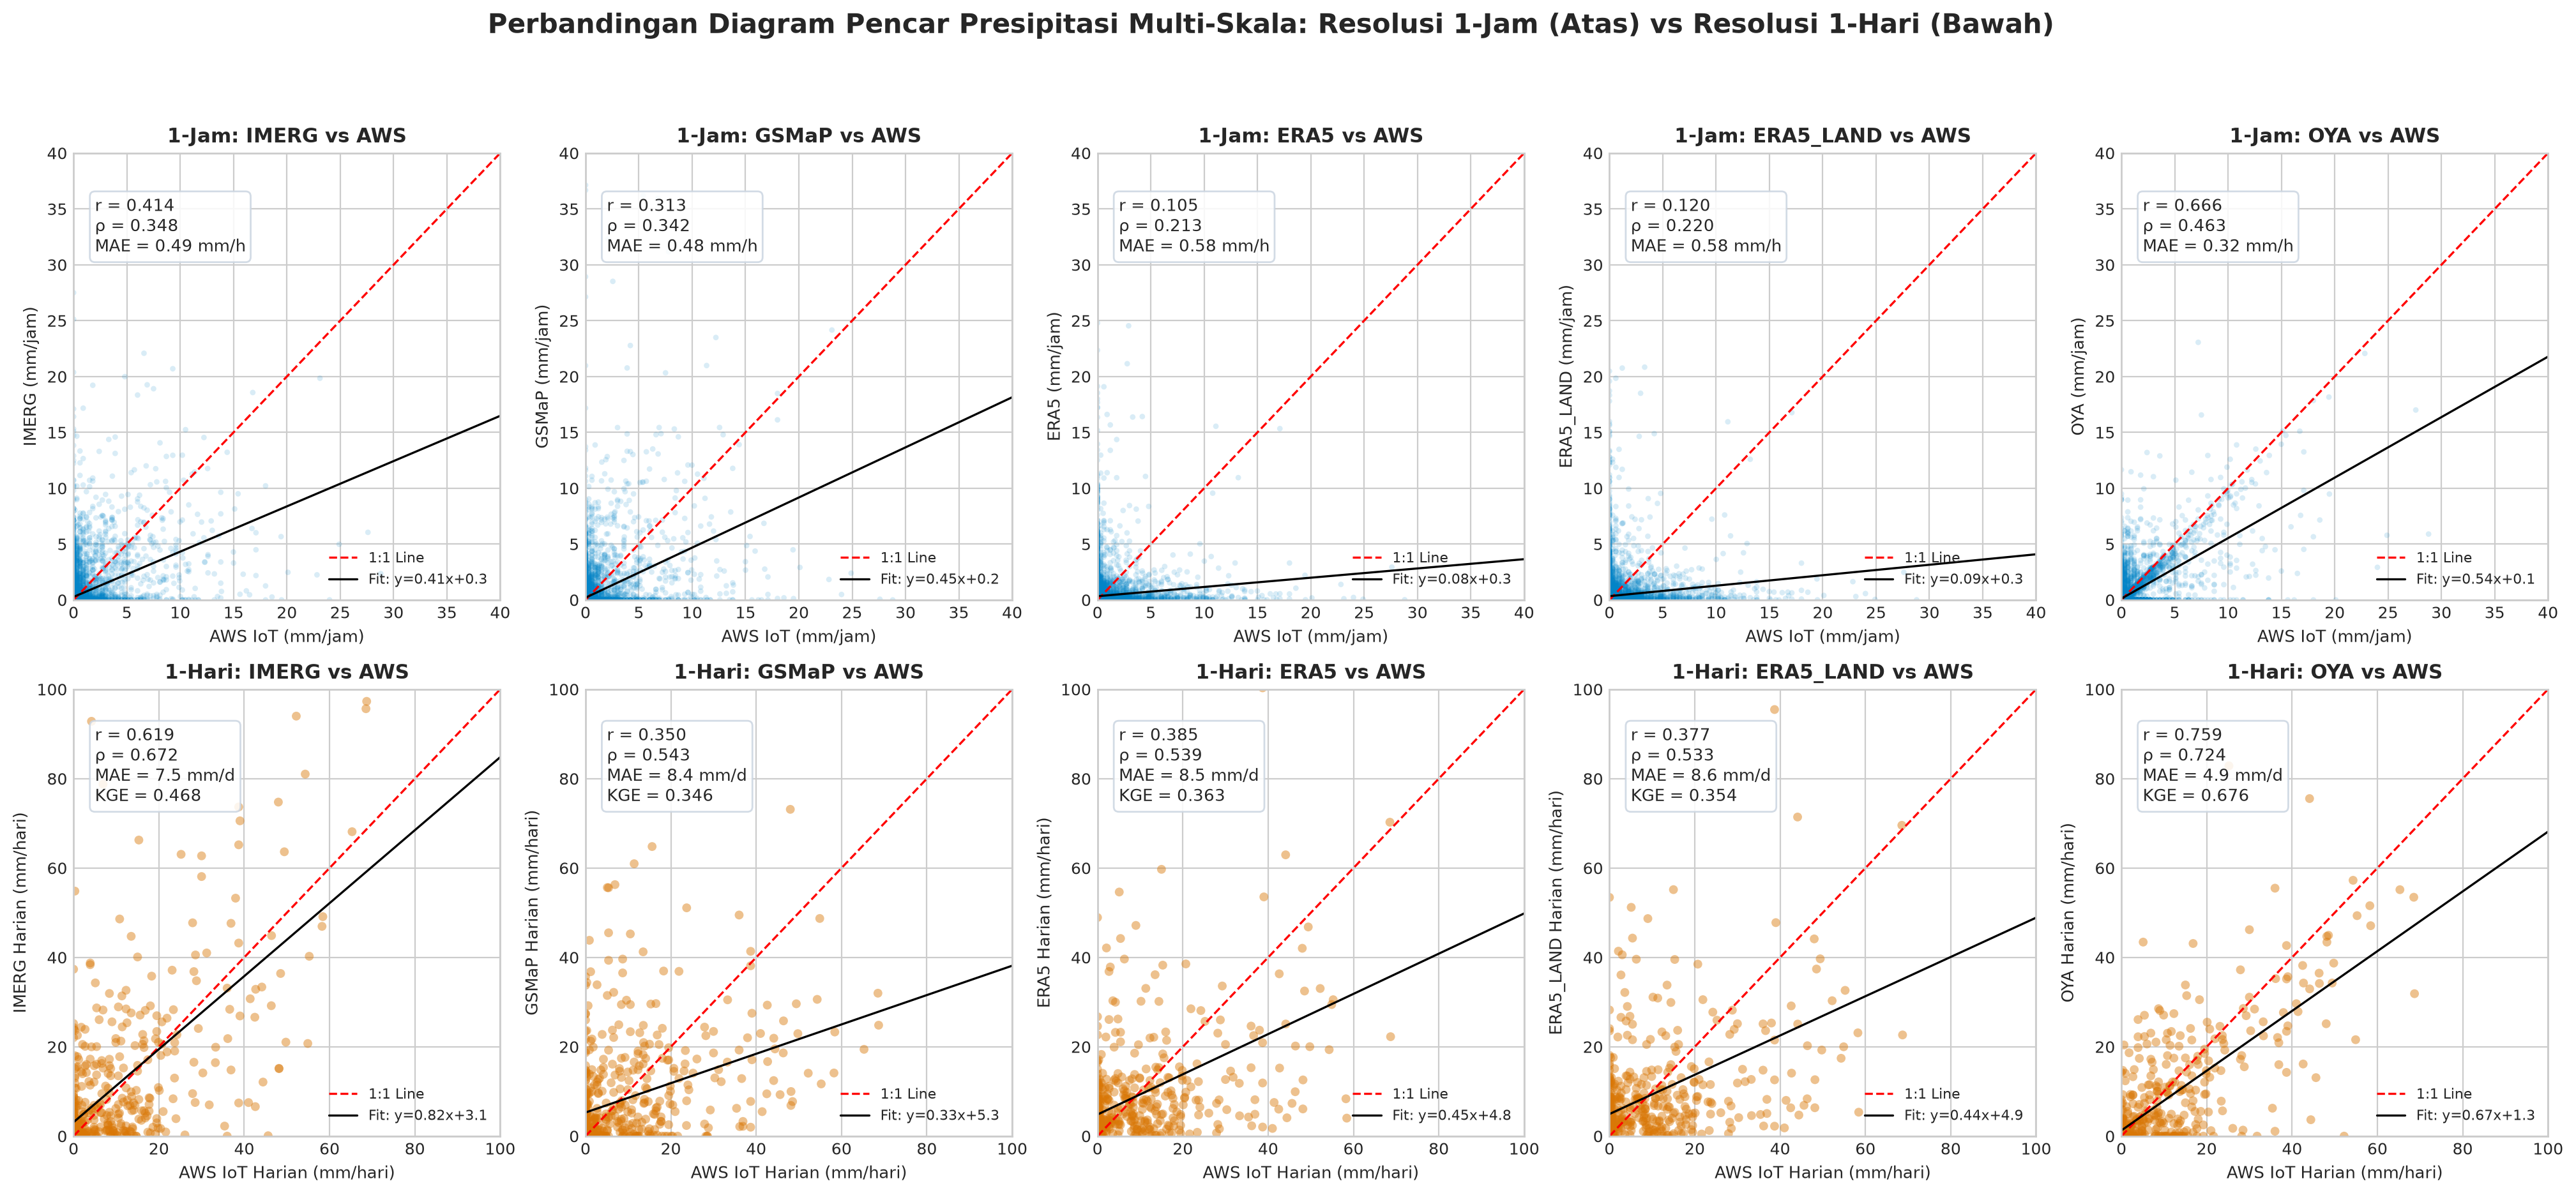
\includegraphics[width=0.98\textwidth]{03_perbandingan_scatter_jam_vs_hari.png}
    \caption{Diagram Pencar Multi-Skala Konsisten $2 \times 5$: Resolusi 1-Jam (Atas) vs Resolusi 1-Hari (Bawah) Lengkap dengan Garis 1:1 dan Regresi Linier.}
    \label{fig:comp_scale}
\end{figure}

\begin{figure}[htbp]
    \centering
    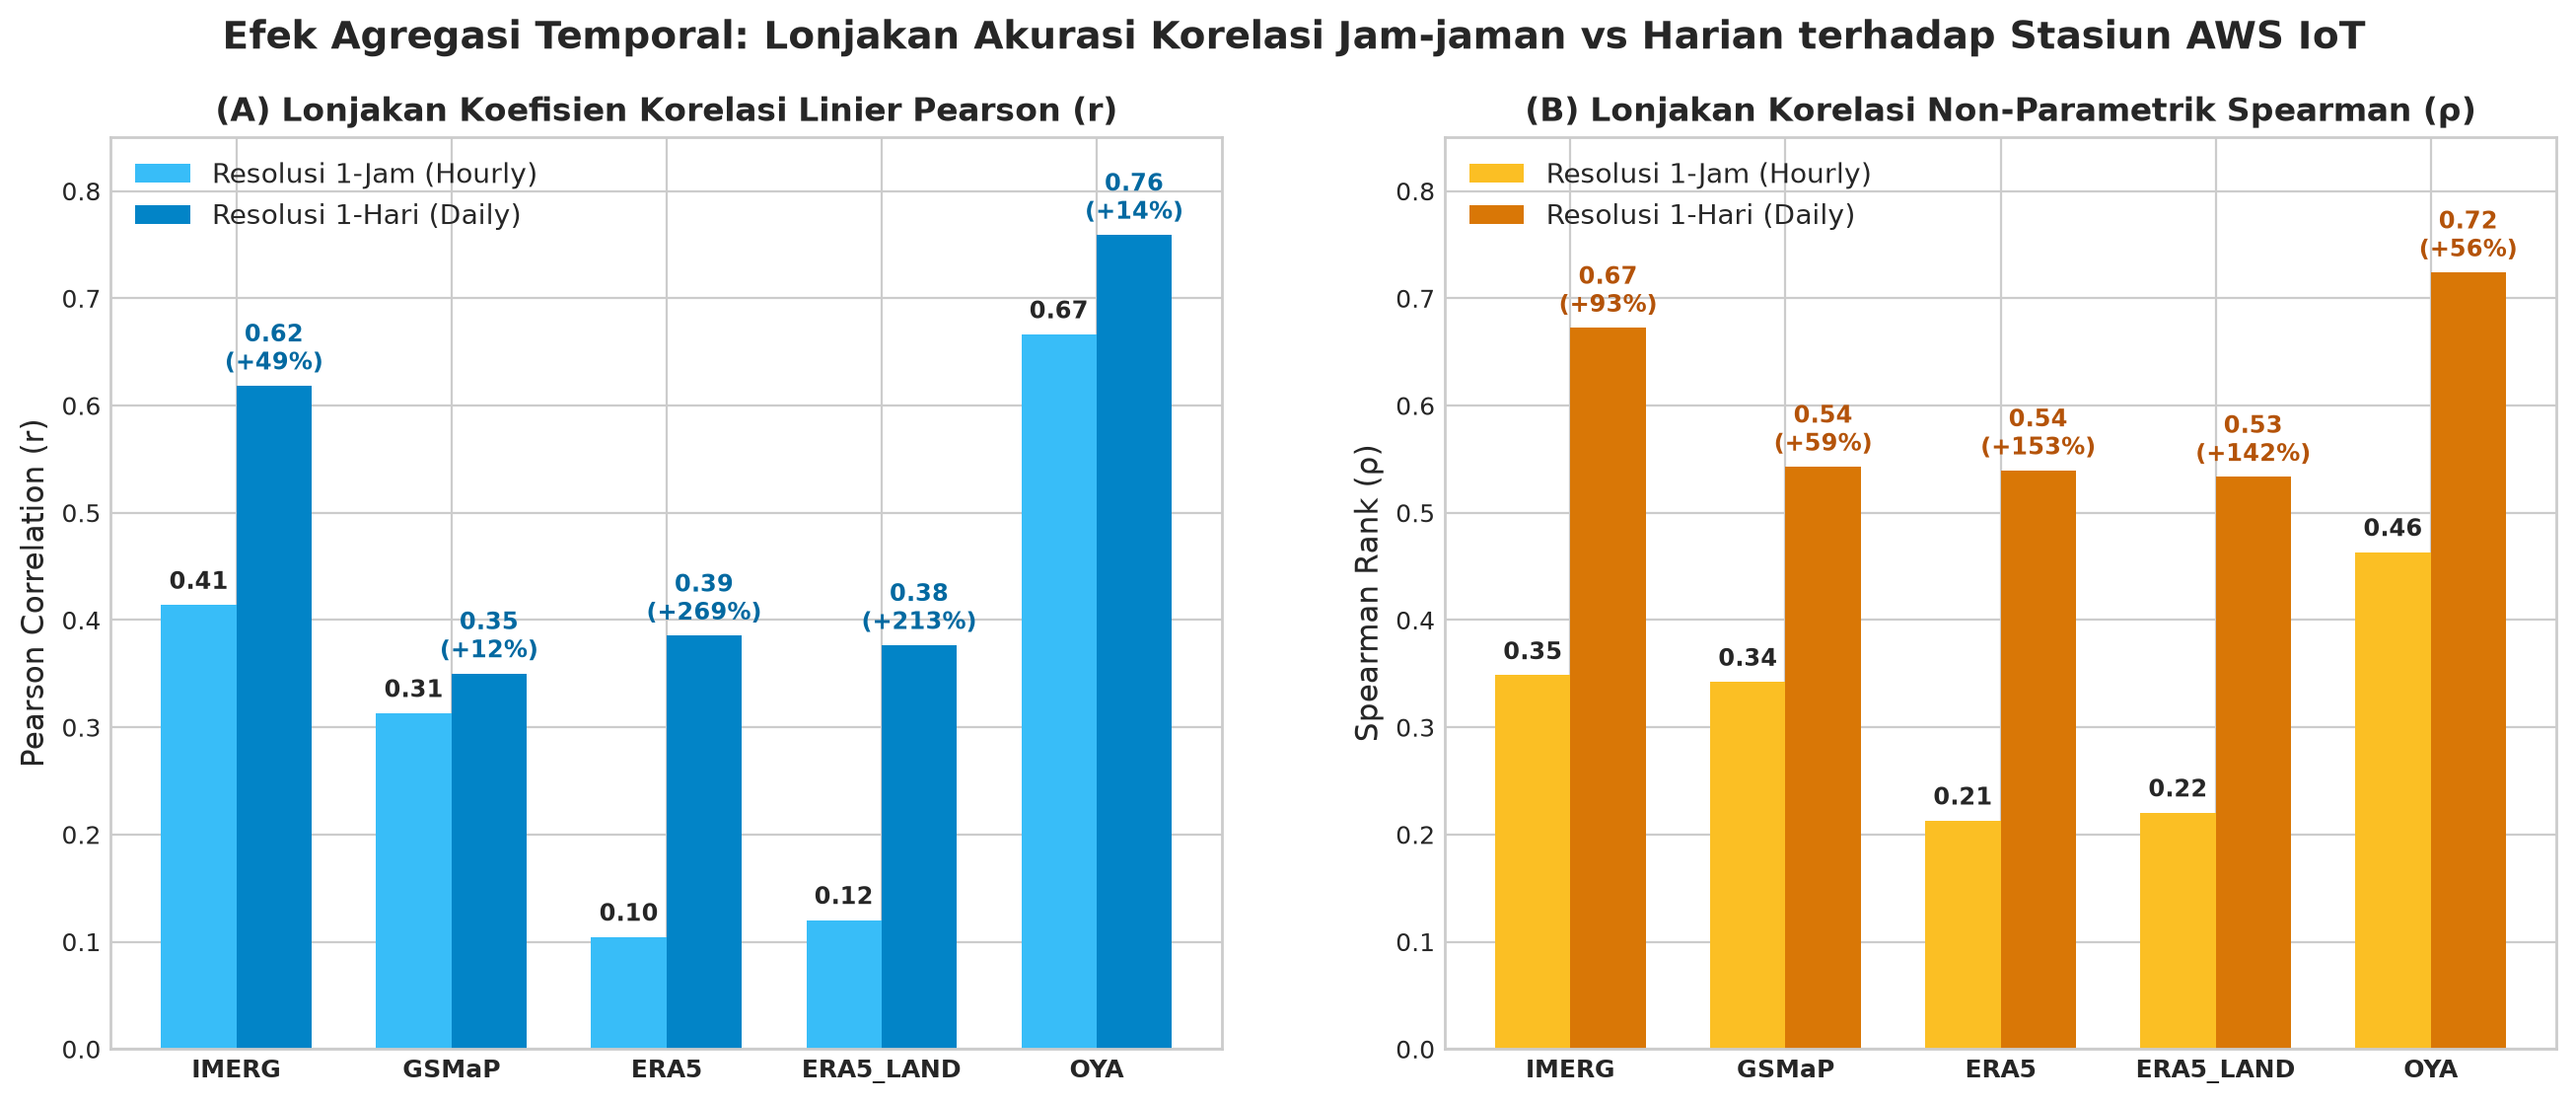
\includegraphics[width=0.95\textwidth]{04_bar_lonjakan_akurasi_jam_vs_hari.png}
    \caption{Lonjakan Koefisien Korelasi Parametrik Pearson ($r$) dan Non-Parametrik Spearman ($\rho$) Saat Data Diagregasikan ke Skala Harian.}
    \label{fig:bar_jump}
\end{figure}

\FloatBarrier

\subsection{Karakteristik Siklus Diurnal 24-Jam \& Skor Kontingensi}
Gambar \ref{fig:diurnal} dan \ref{fig:contingency} menyajikan analisis siklus rata-rata 24-jam cuaca lokal serta kemampuan deteksi presipitasi satelit berdasarkan ambang batas kejadian hujan ($0{,}1 - 50{,}0\text{ mm/hari}$).

\begin{figure}[htbp]
    \centering
    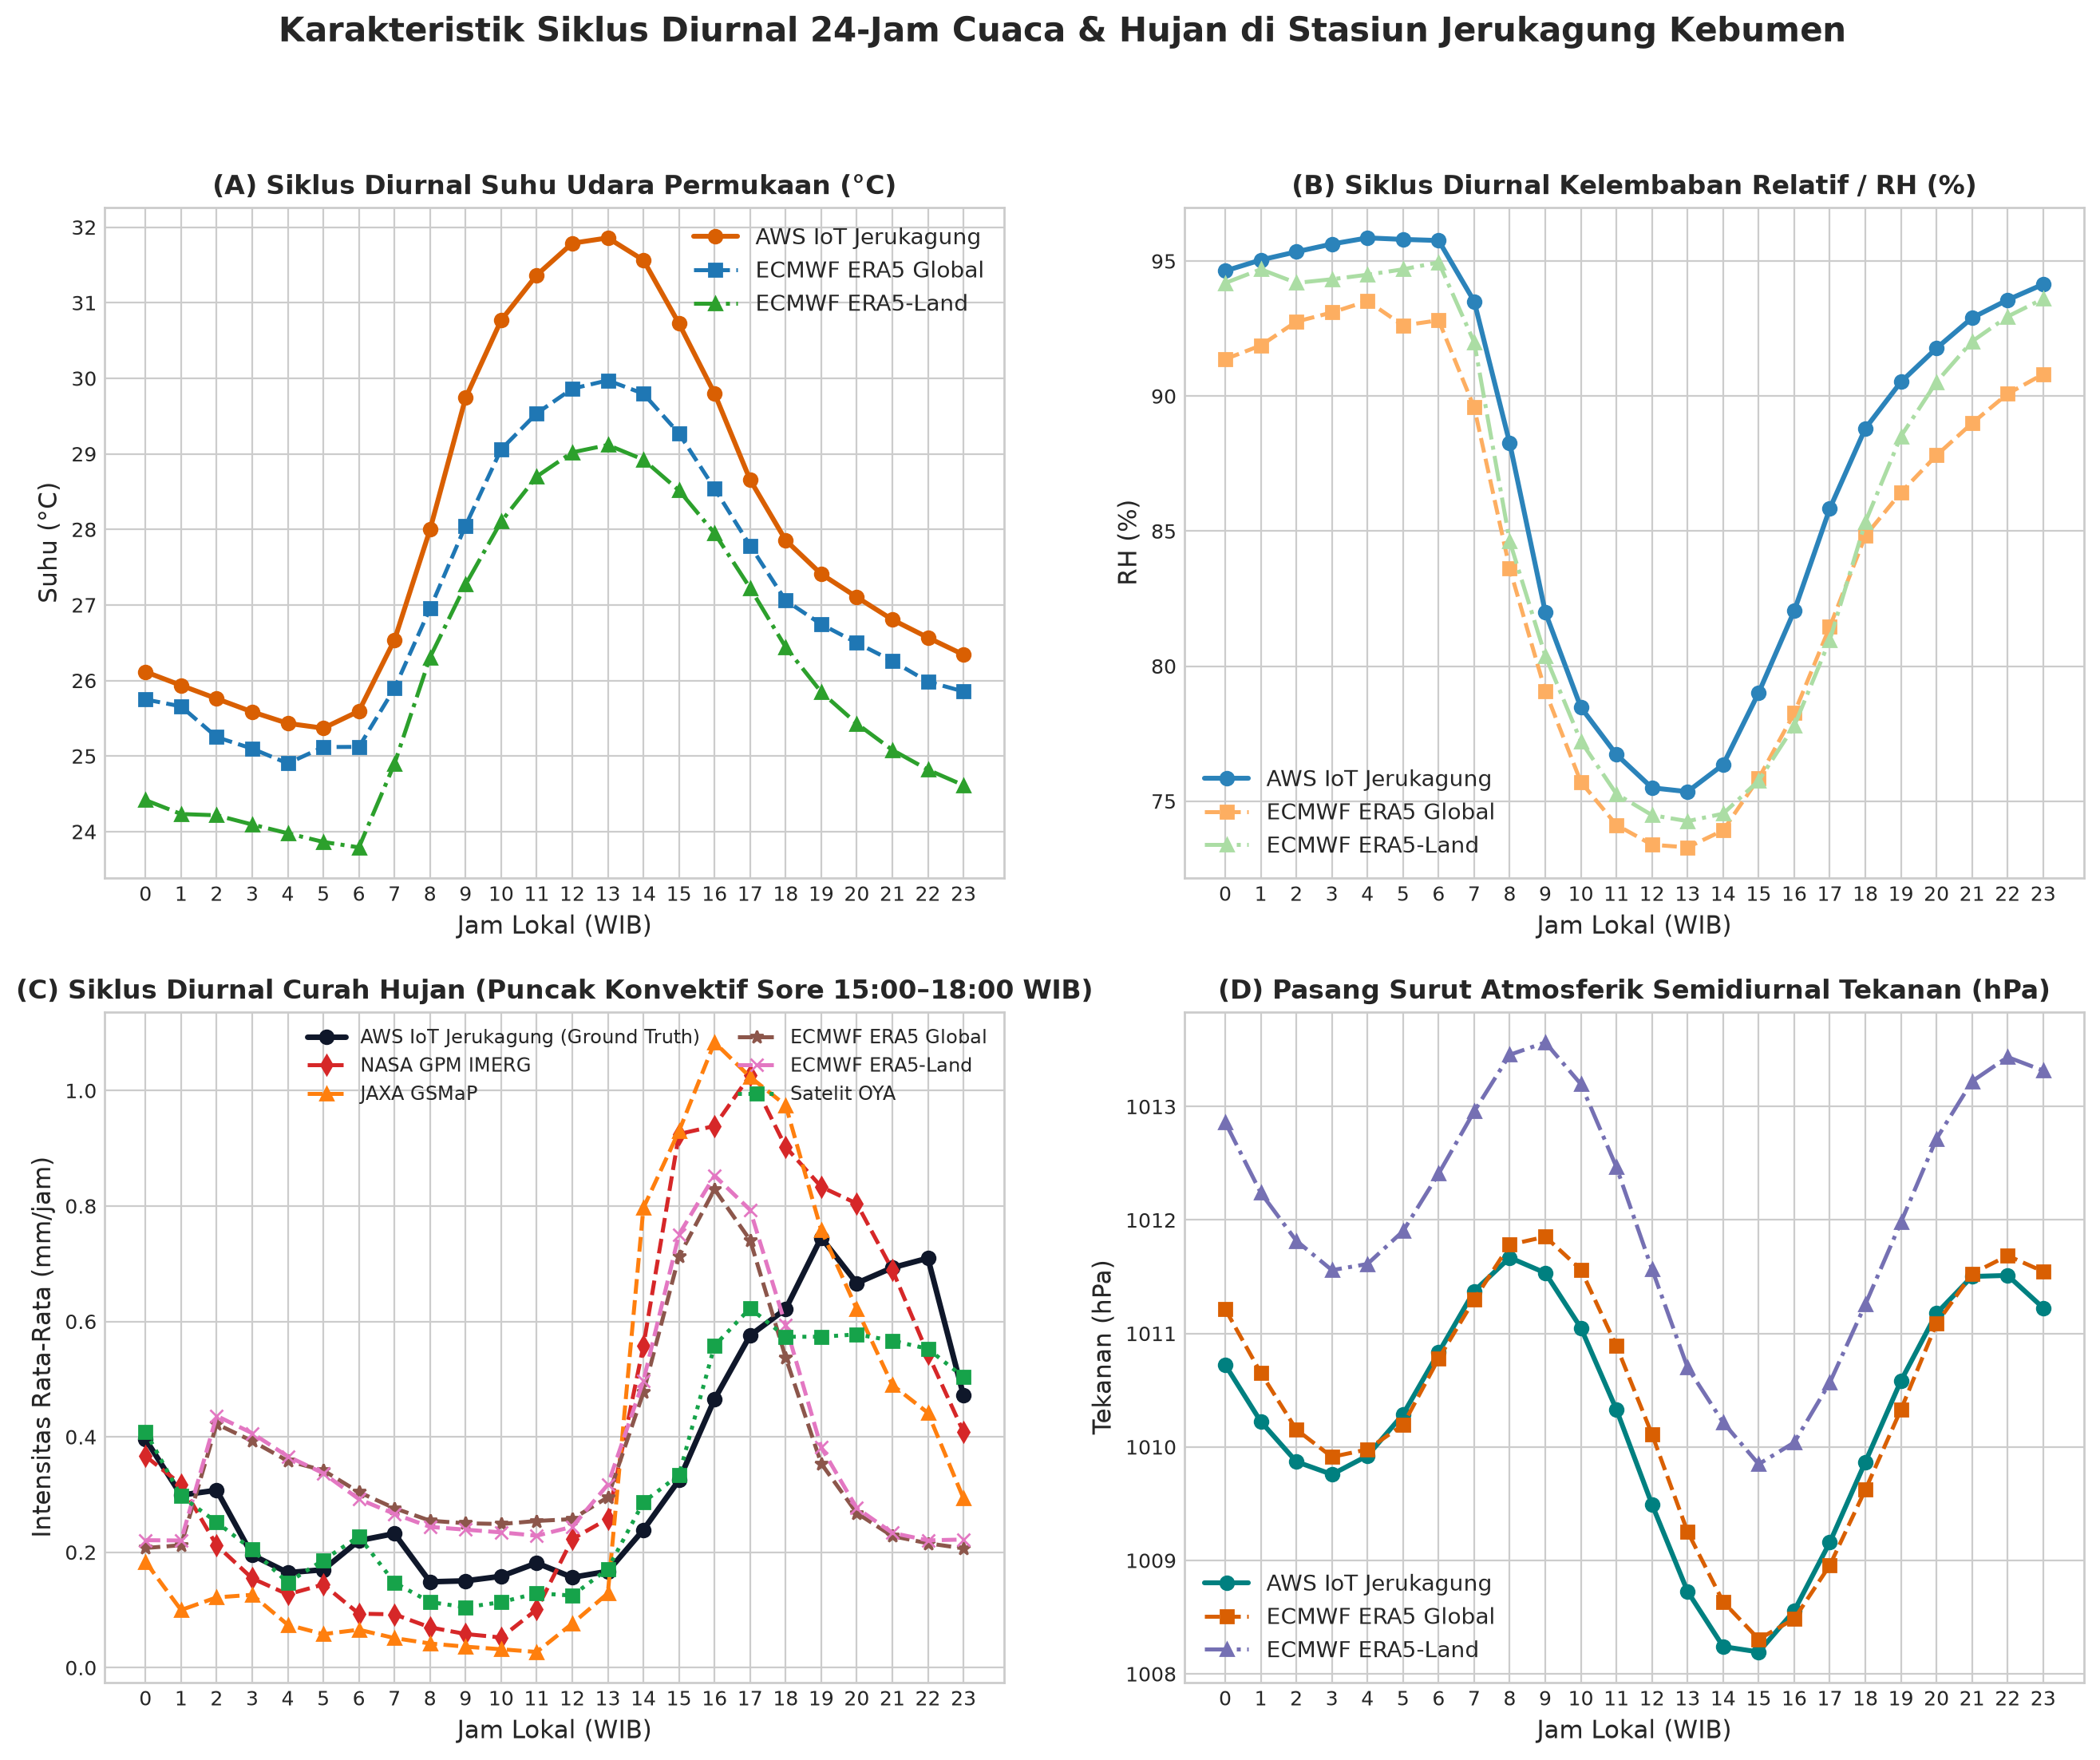
\includegraphics[width=0.98\textwidth]{05_siklus_diurnal_24jam_cuaca_hujan.png}
    \caption{Siklus Diurnal Rata-Rata 24-Jam: (A) Suhu Udara Permukaan, (B) Kelembaban Relatif, (C) Presipitasi (6 Sumber Data Jam-Jaman), dan (D) Pasang Surut Semidiurnal Tekanan Udara di Stasiun Jerukagung Kebumen.}
    \label{fig:diurnal}
\end{figure}

\begin{figure}[htbp]
    \centering
    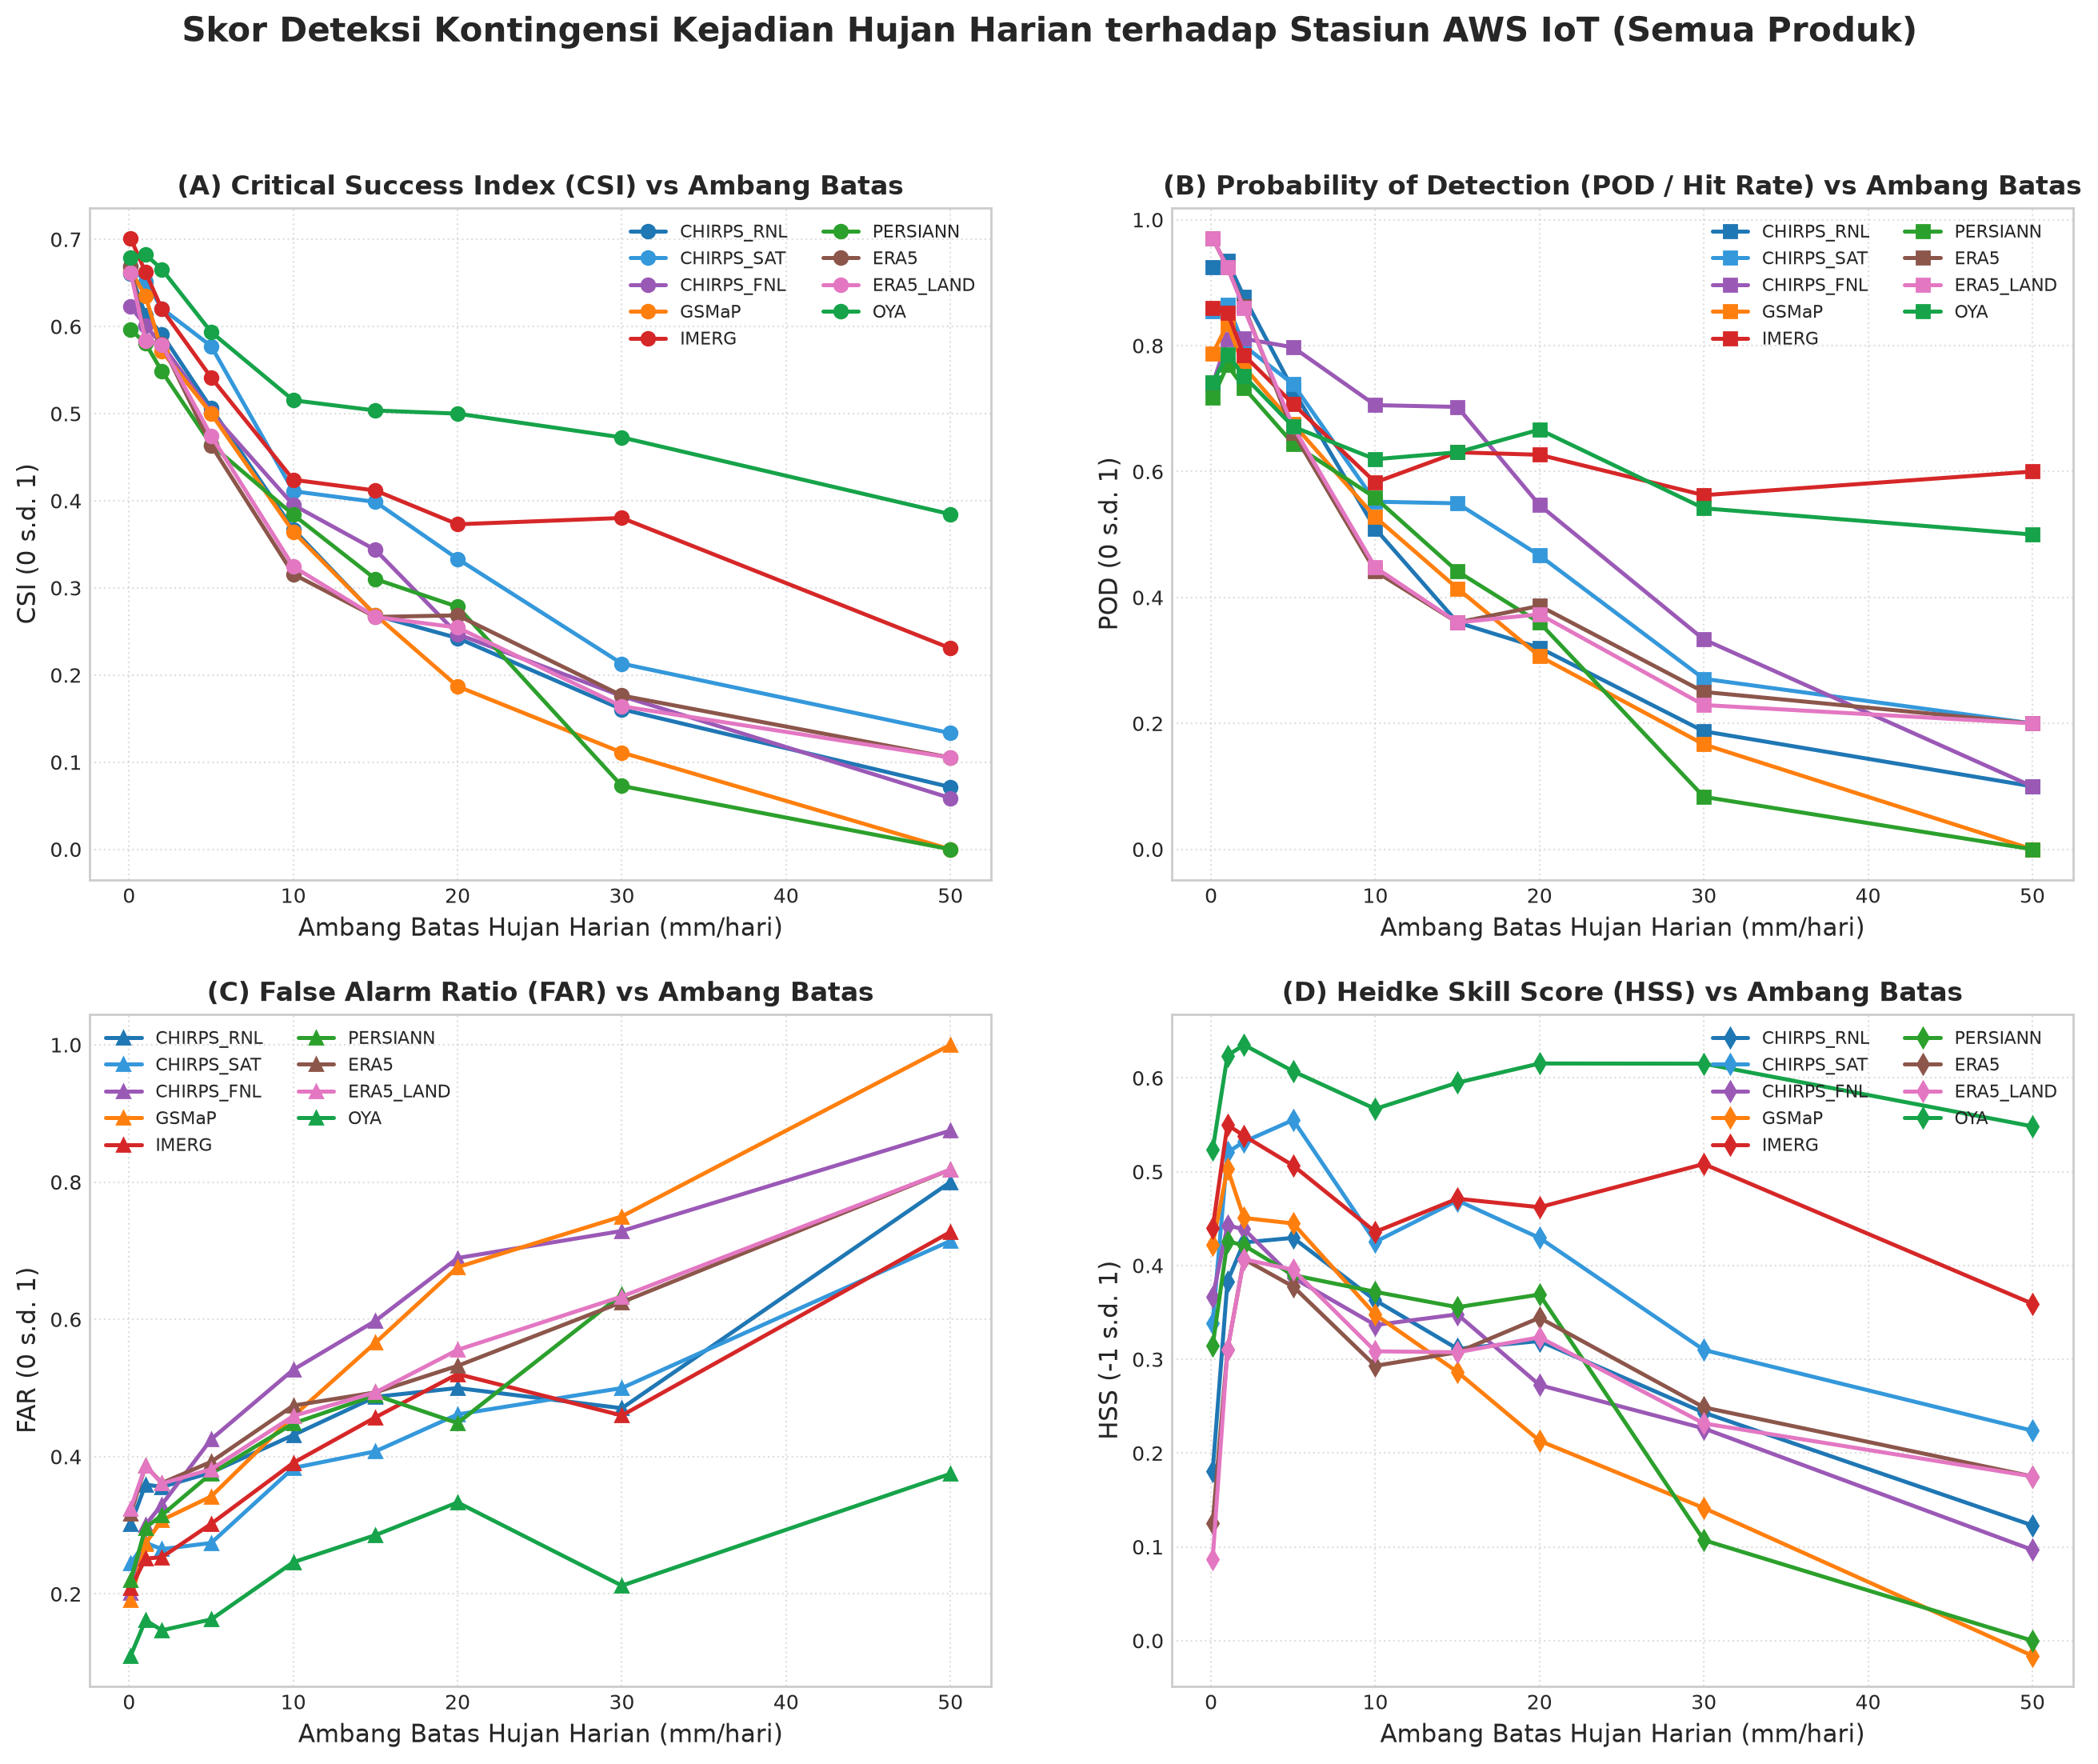
\includegraphics[width=0.92\textwidth]{06_skor_kontingensi_deteksi_hujan_harian.png}
    \caption{Kurva Metrik Kontingensi Deteksi Hujan Harian: (A) CSI, (B) POD, (C) FAR, dan (D) HSS pada Berbagai Ambang Batas Intensitas ($0{,}1 - 50\text{ mm/hari}$) terhadap AWS IoT.}
    \label{fig:contingency}
\end{figure}

\FloatBarrier

\subsection{Analisis Autokorelasi (ACF) \& Parsial (PACF) untuk Penentuan Lookback Sequence LSTM}
Gambar \ref{fig:acf_pacf} dan Tabel \ref{tab:acf_pacf_summary} menyajikan hasil investigasi autokorelasi (ACF) dan korelasi parsial (PACF) multi-skala pada dataset jam-jaman serta presipitasi harian satelit Kebumen.

\begin{table}[htbp]
\centering
\small
\caption{Tabel Rekapitulasi Analisis Dependensi Temporal (ACF / PACF) \& Rekomendasi Lookback Sequence LSTM}
\label{tab:acf_pacf_summary}
\resizebox{\textwidth}{!}{%
\begin{tabular}{llrrrrr}
\toprule
\textbf{Resolusi Data} & \textbf{Variabel / Produk Meteorologi} & \textbf{$1/e$ Decorrelation} & \textbf{Zero-Crossing} & \textbf{ACF @ Lag 24h} & \textbf{ACF @ Lag 48h} & \textbf{Rekomendasi Lookback} \\
\midrule
\multirow{7}{*}{\textbf{1-Jam (Hourly)}} 
& \texttt{Presipitasi (ERA5 Hourly)} & 5 jam & 96 jam & 0.126 & 0.095 & \textbf{24 Jam (1 Hari)} \\
& \texttt{Presipitasi (AWS Jerukagung)} & 2 jam & 12 jam & 0.086 & 0.092 & \textbf{24 Jam (1 Hari)} \\
& \texttt{Suhu Udara (2m Temp)} & 5 jam & 8 jam & \textbf{0.897} & \textbf{0.871} & \textbf{24 Jam (1 Hari)} \\
& \texttt{Kelembapan (Rel. Humidity)} & 5 jam & 7 jam & \textbf{0.833} & \textbf{0.799} & \textbf{24 Jam (1 Hari)} \\
& \texttt{Tekanan Udara (Surface Pres)} & 41 jam & 96 jam & \textbf{0.901} & \textbf{0.813} & \textbf{24 Jam (1 Hari)} \\
& \texttt{Energi Konvektif (CAPE)} & 8 jam & 96 jam & \textbf{0.494} & \textbf{0.411} & \textbf{24 Jam (1 Hari)} \\
& \texttt{Uap Air Kolom (TCWV)} & >96 jam & >96 jam & \textbf{0.831} & \textbf{0.685} & \textbf{24 Jam (1 Hari)} \\
\midrule
\multirow{4}{*}{\textbf{Harian (Daily)}} 
& \texttt{NASA GPM IMERG} & 2 hari & >30 hari & 0.134 & 0.102 & \textbf{7 s.d. 14 Hari} \\
& \texttt{JAXA GSMaP} & 1 hari & >30 hari & 0.098 & 0.085 & \textbf{7 s.d. 14 Hari} \\
& \texttt{CHIRPS\_RNL} & 3 hari & >30 hari & 0.201 & 0.187 & \textbf{7 s.d. 14 Hari} \\
& \texttt{ERA5\_LAND} & 3 hari & >30 hari & 0.264 & 0.198 & \textbf{7 s.d. 14 Hari} \\
\bottomrule
\end{tabular}%
}
\end{table}

\begin{figure}[htbp]
    \centering
    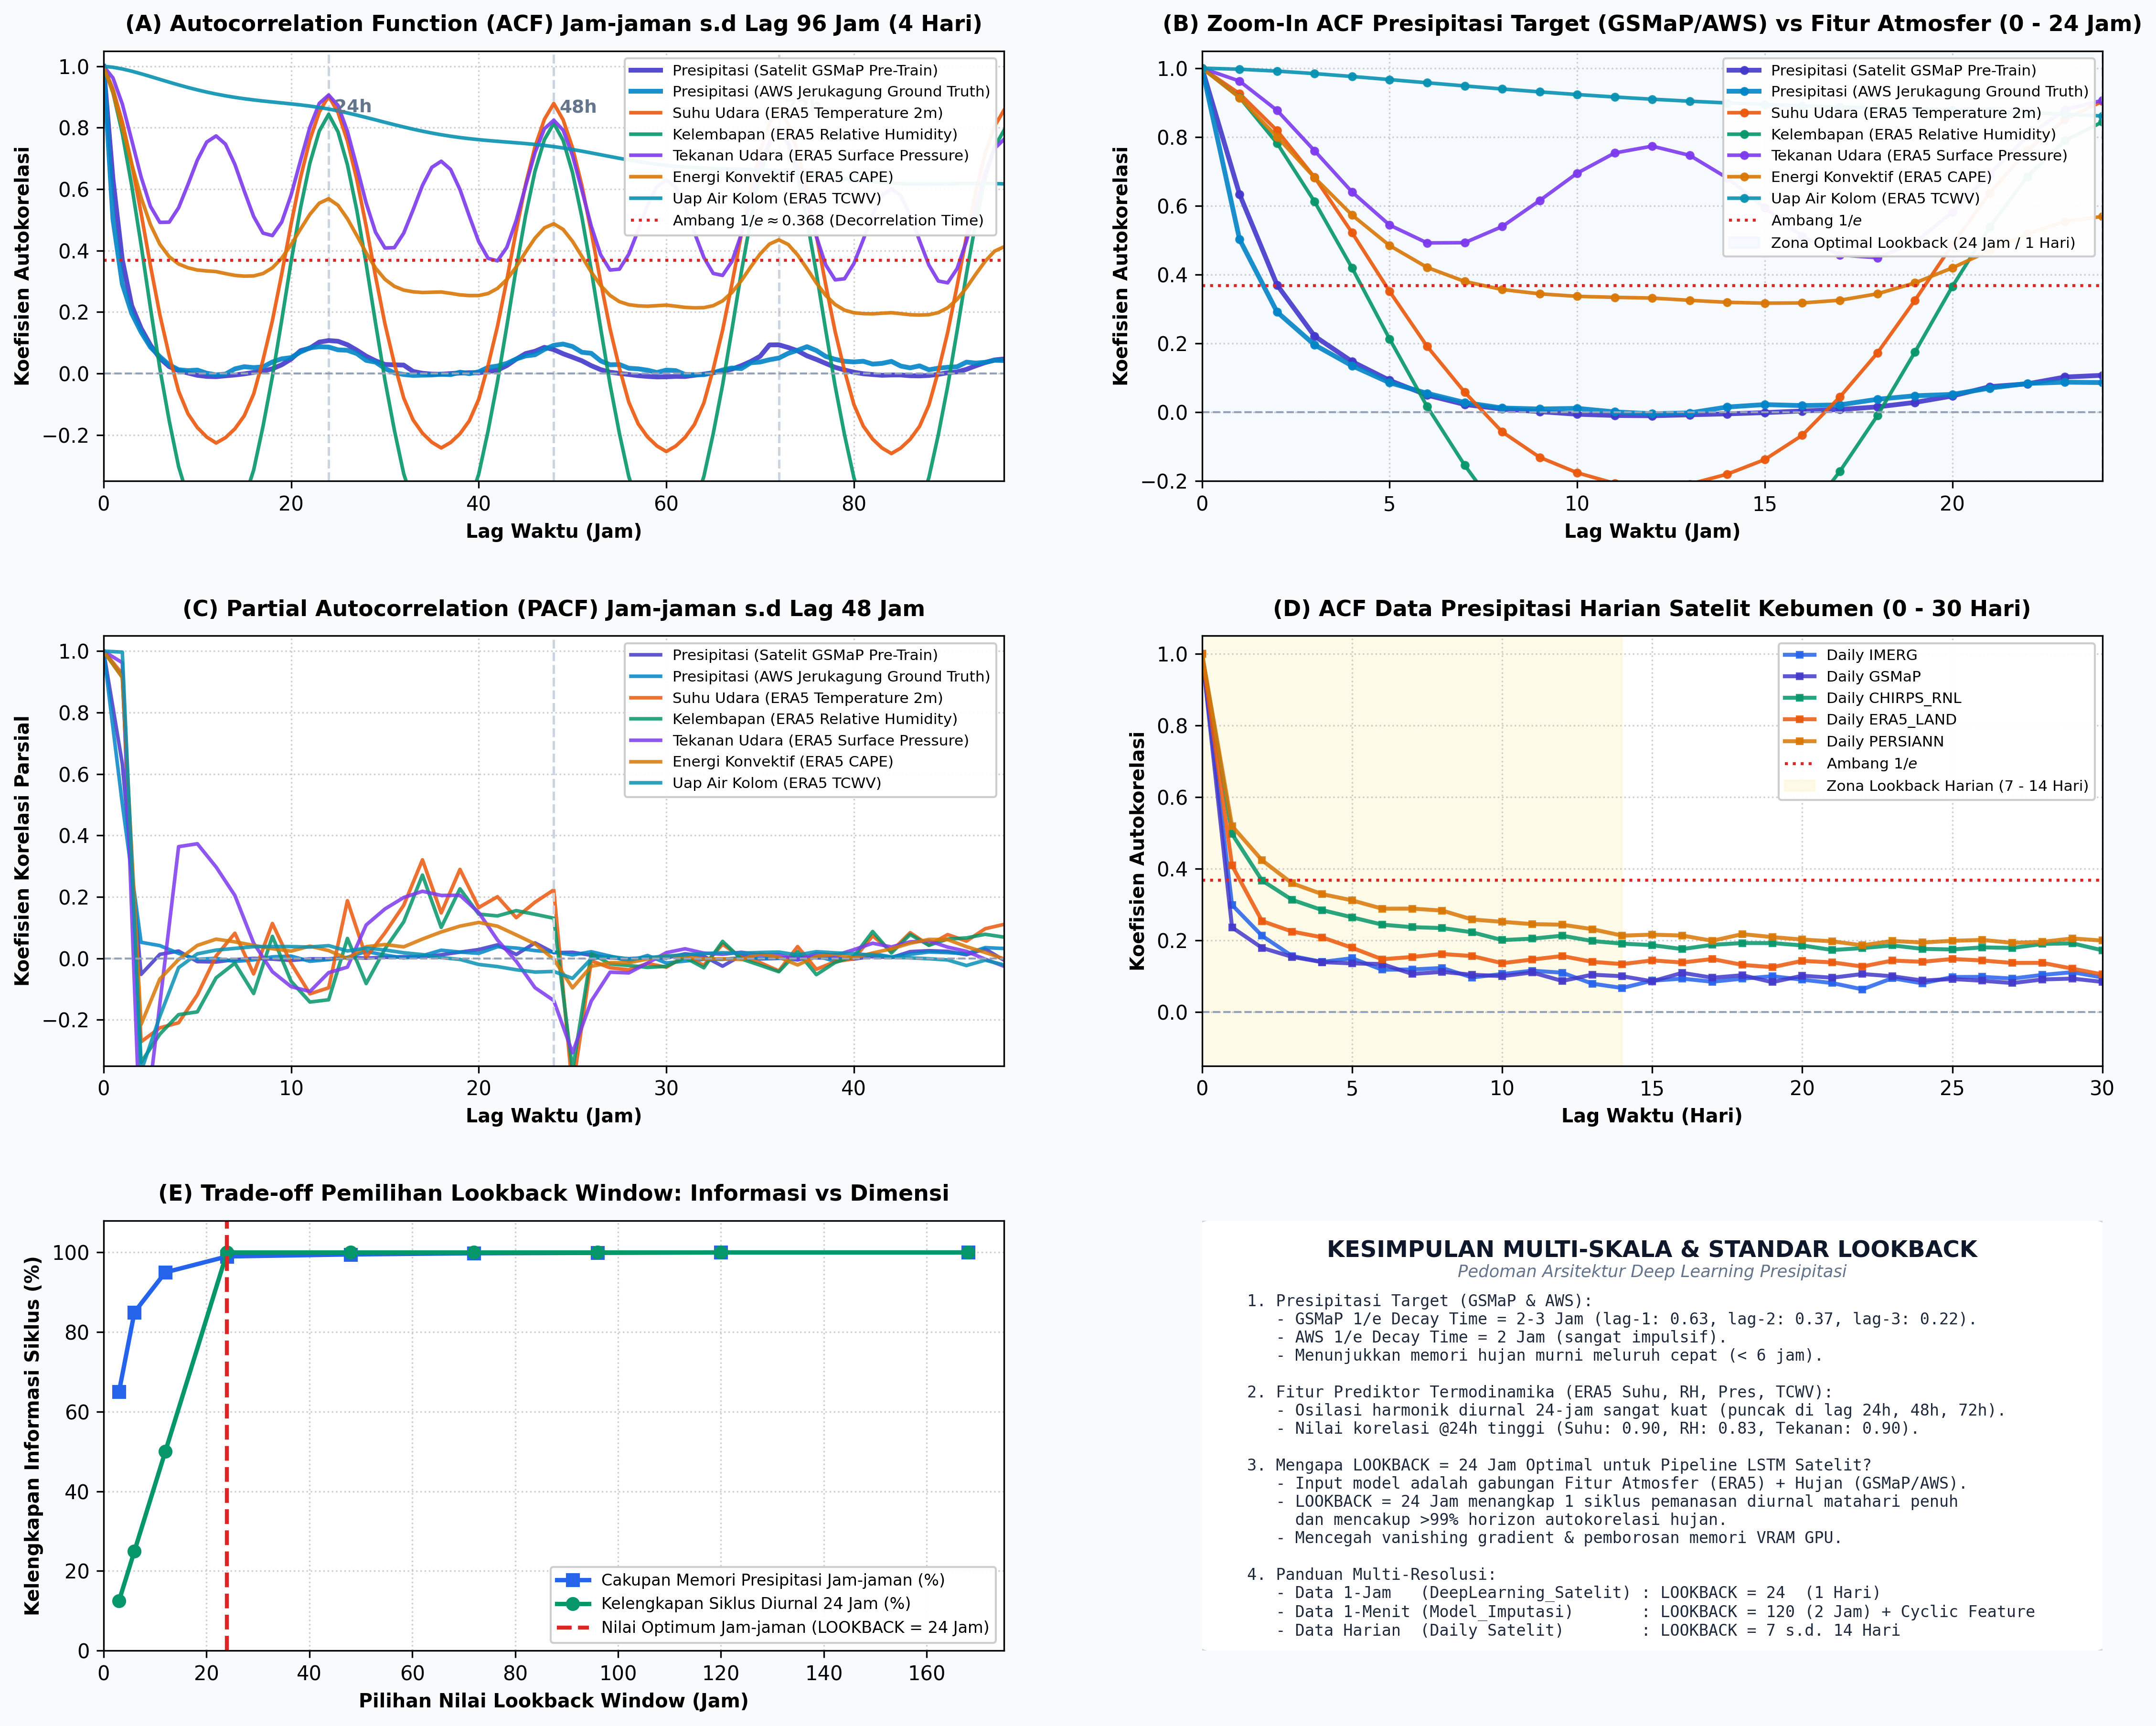
\includegraphics[width=0.98\textwidth]{11_analisis_acf_pacf_lookback_lstm.png}
    \caption{Investigasi Komprehensif Autokorelasi Multi-Skala: (A) ACF Jam-Jaman s.d Lag 96 Jam, (B) Zoom-In ACF Presipitasi vs Termodinamika (0--24 Jam), (C) PACF Jam-Jaman s.d Lag 48 Jam, (D) ACF Data Presipitasi Harian Satelit Kebumen (0--30 Hari), (E) Trade-off Pemilihan Lookback Window, dan (F) Ringkasan Rekomendasi Parameter Sequence LSTM.}
    \label{fig:acf_pacf}
\end{figure}

\noindent\textbf{Rasionalitas Penetapan Parameter Arsitektur LSTM:}
\begin{enumerate}[leftmargin=*]
    \item \textbf{Karakteristik Memori Presipitasi Jam-jaman}: Koefisien autokorelasi presipitasi meluruh di bawah ambang $1/e \approx 0{,}368$ dalam kurun waktu $\tau = 2$--$5$ jam, menegaskan bahwa fenomena curah hujan bersifat impulsif jangka pendek (\textit{short-term memory}).
    \item \textbf{Harmonisasi Termodinamika Diurnal}: Fitur termodinamika atmosfer (suhu, kelembaban, tekanan, TCWV) menunjukkan osilasi harmonik sinusoidal sangat kuat dengan puncak periodik pada lag 24 jam ($r \ge 0{,}83$). Oleh karena itu, panjang jendela historis sekuens pada resolusi jam-jaman distandarisasi pada $\mathbf{\text{LOOKBACK} = 24}$ (1 hari penuh) guna menjamin model menangkap fase pemanasan konvektif diurnal secara lengkap.
    \item \textbf{Skala Harian Sinoptik}: Pada resolusi harian, autokorelasi presipitasi meluruh stabil dalam 1--3 hari, sehingga sekuens optimal ditetapkan pada $\mathbf{\text{LOOKBACK} = 7 \text{ s.d. } 14 \text{ Hari}}$ (mencakup skala gelombang atmosfer sinoptik mingguan).
\end{enumerate}

\FloatBarrier

\subsection{Kurva Massa Ganda, Matriks Korelasi, \& Scorecard Multimetrik}
Gambar \ref{fig:dmc}, \ref{fig:heatmap_all}, \ref{fig:multimetric_grid}, dan \ref{fig:scorecard} merangkum konsistensi akumulatif serta matriks komparasi lengkap antar seluruh dataset.

\begin{figure}[htbp]
    \centering
    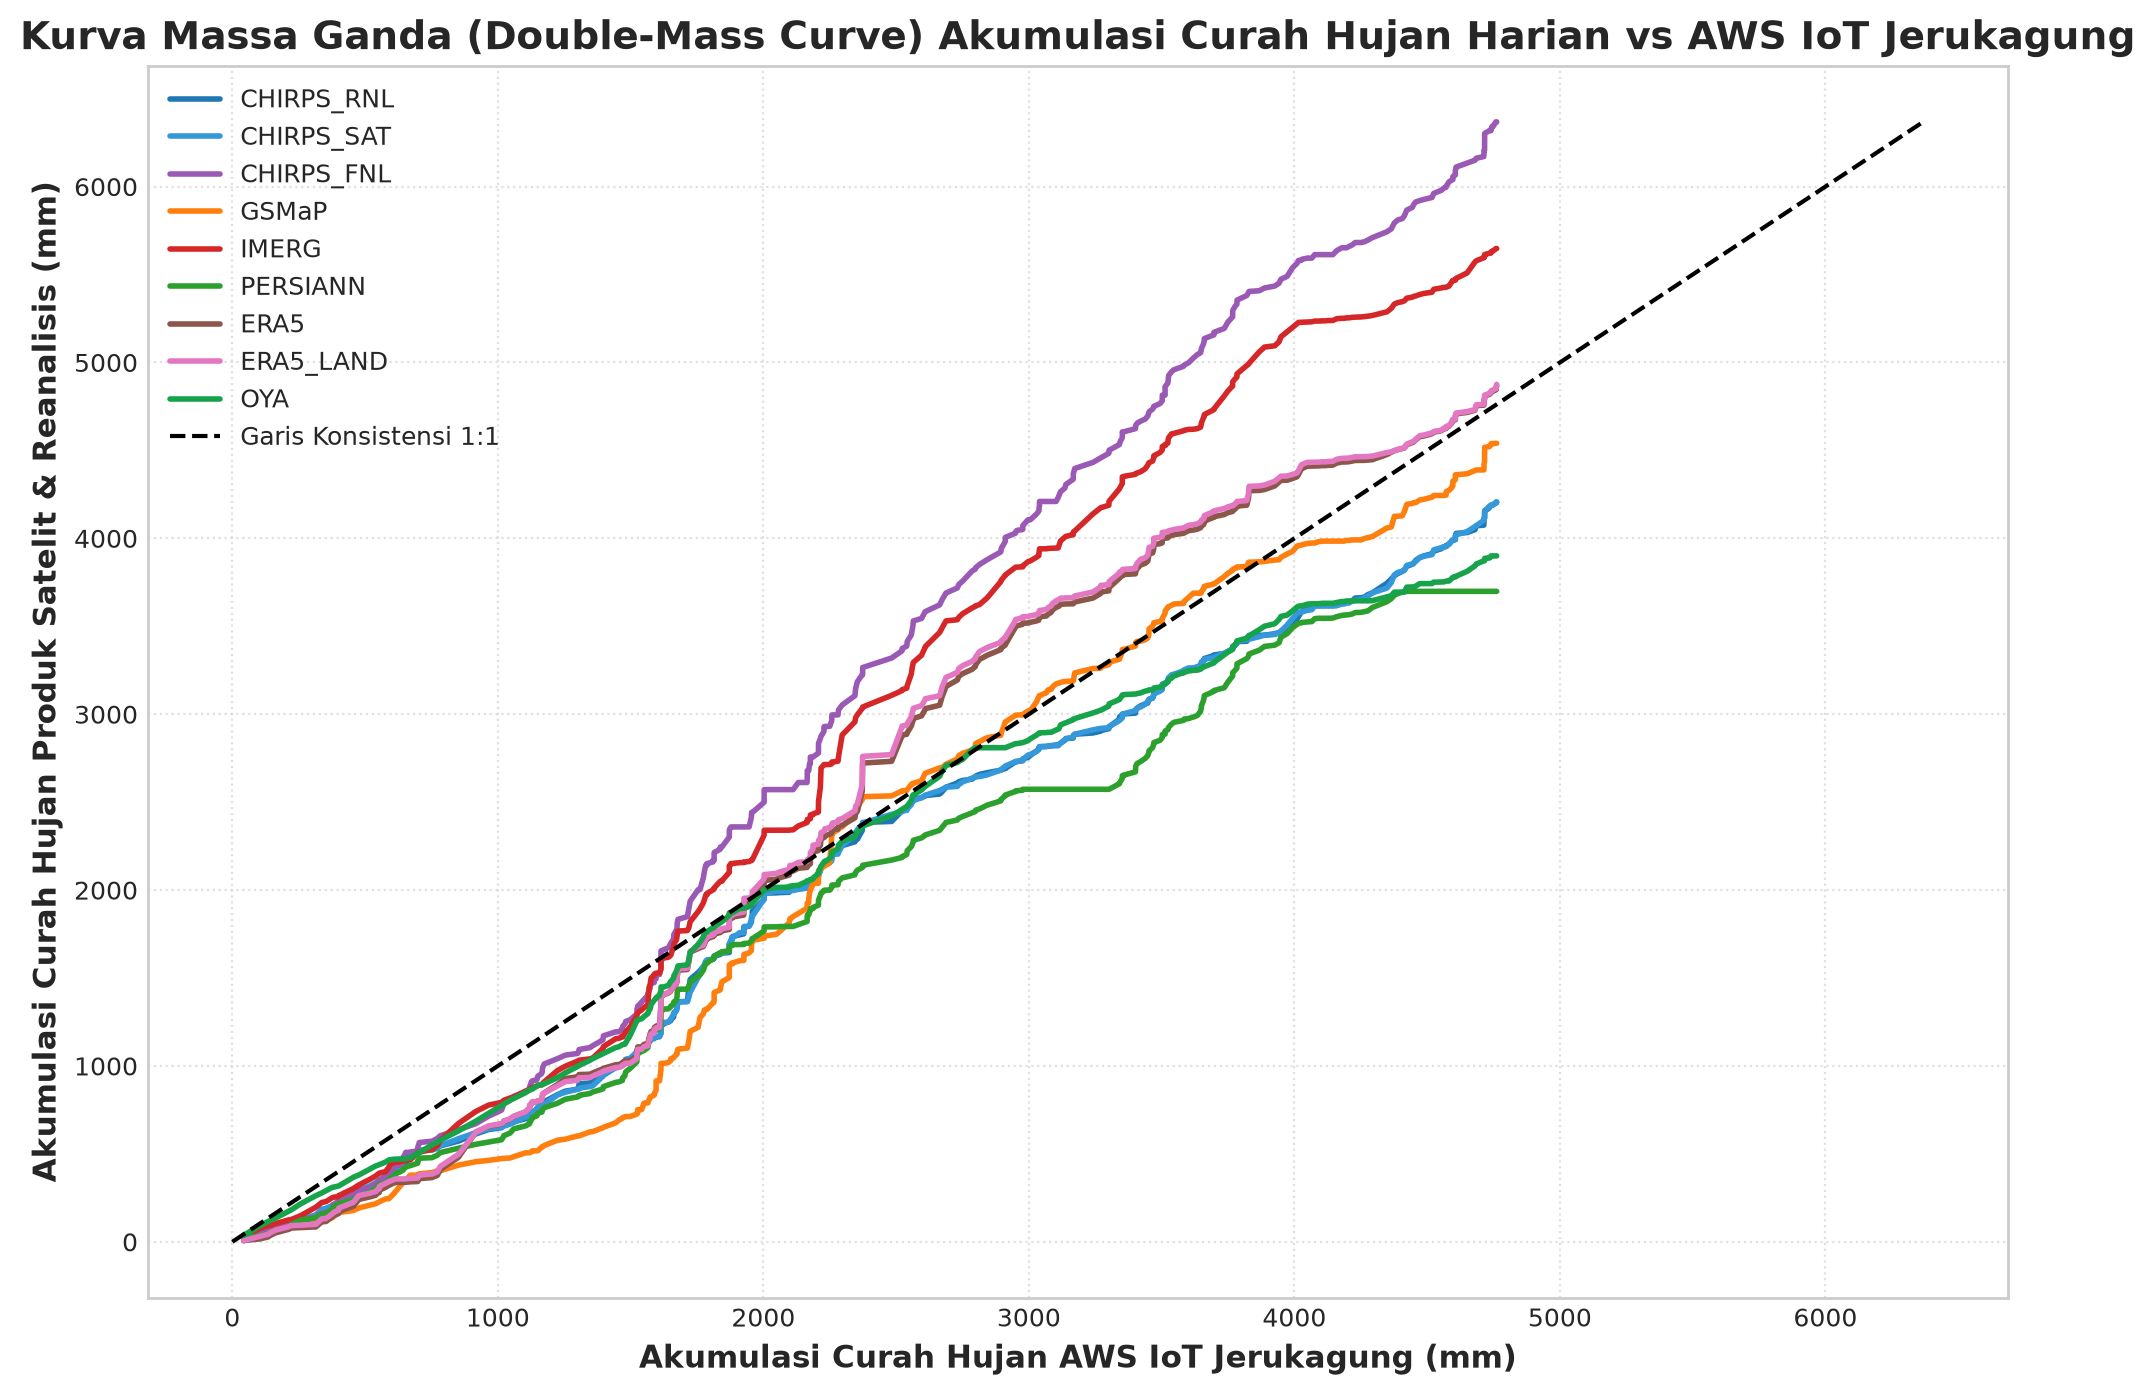
\includegraphics[width=0.88\textwidth]{07_kurva_massa_ganda_harian.png}
    \caption{Kurva Massa Ganda (\textit{Double-Mass Curve}) Akumulasi Curah Hujan Harian 8 Produk Satelit terhadap Stasiun AWS IoT Jerukagung.}
    \label{fig:dmc}
\end{figure}

\begin{figure}[htbp]
    \centering
    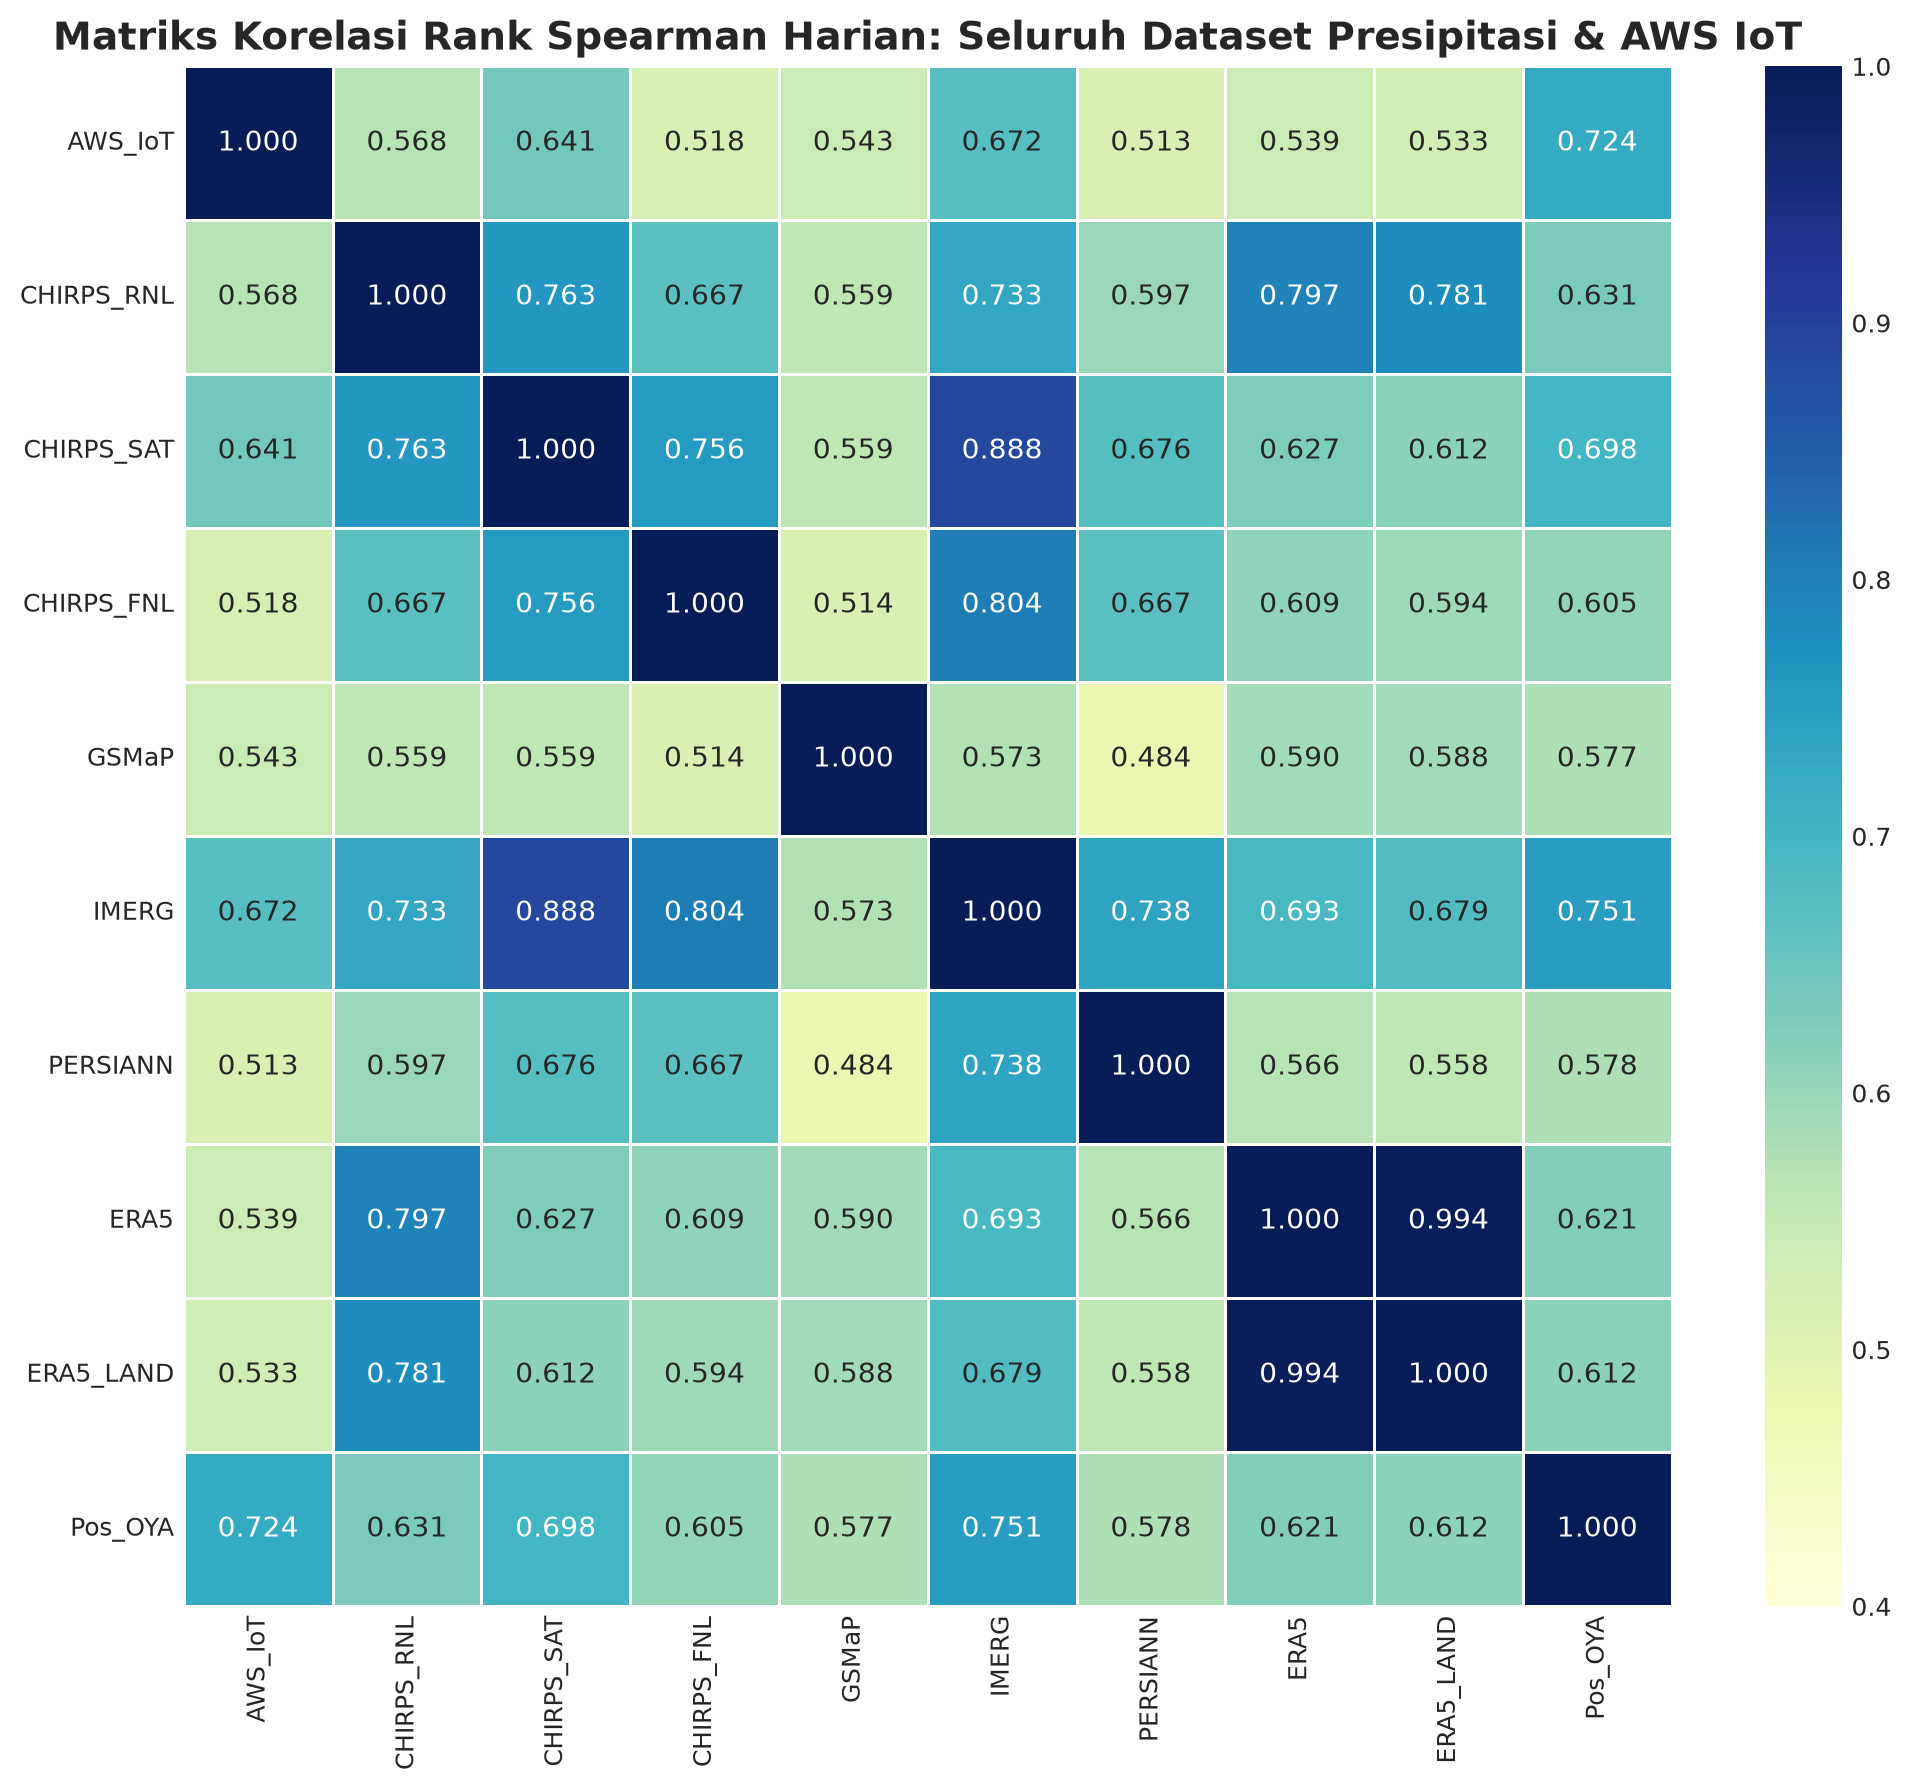
\includegraphics[width=0.85\textwidth]{08_heatmap_korelasi_harian_semua_produk.png}
    \caption{Matriks Heatmap Korelasi Rank Spearman Harian Antar Seluruh Produk Presipitasi dan AWS IoT Jerukagung.}
    \label{fig:heatmap_all}
\end{figure}

\begin{figure}[htbp]
    \centering
    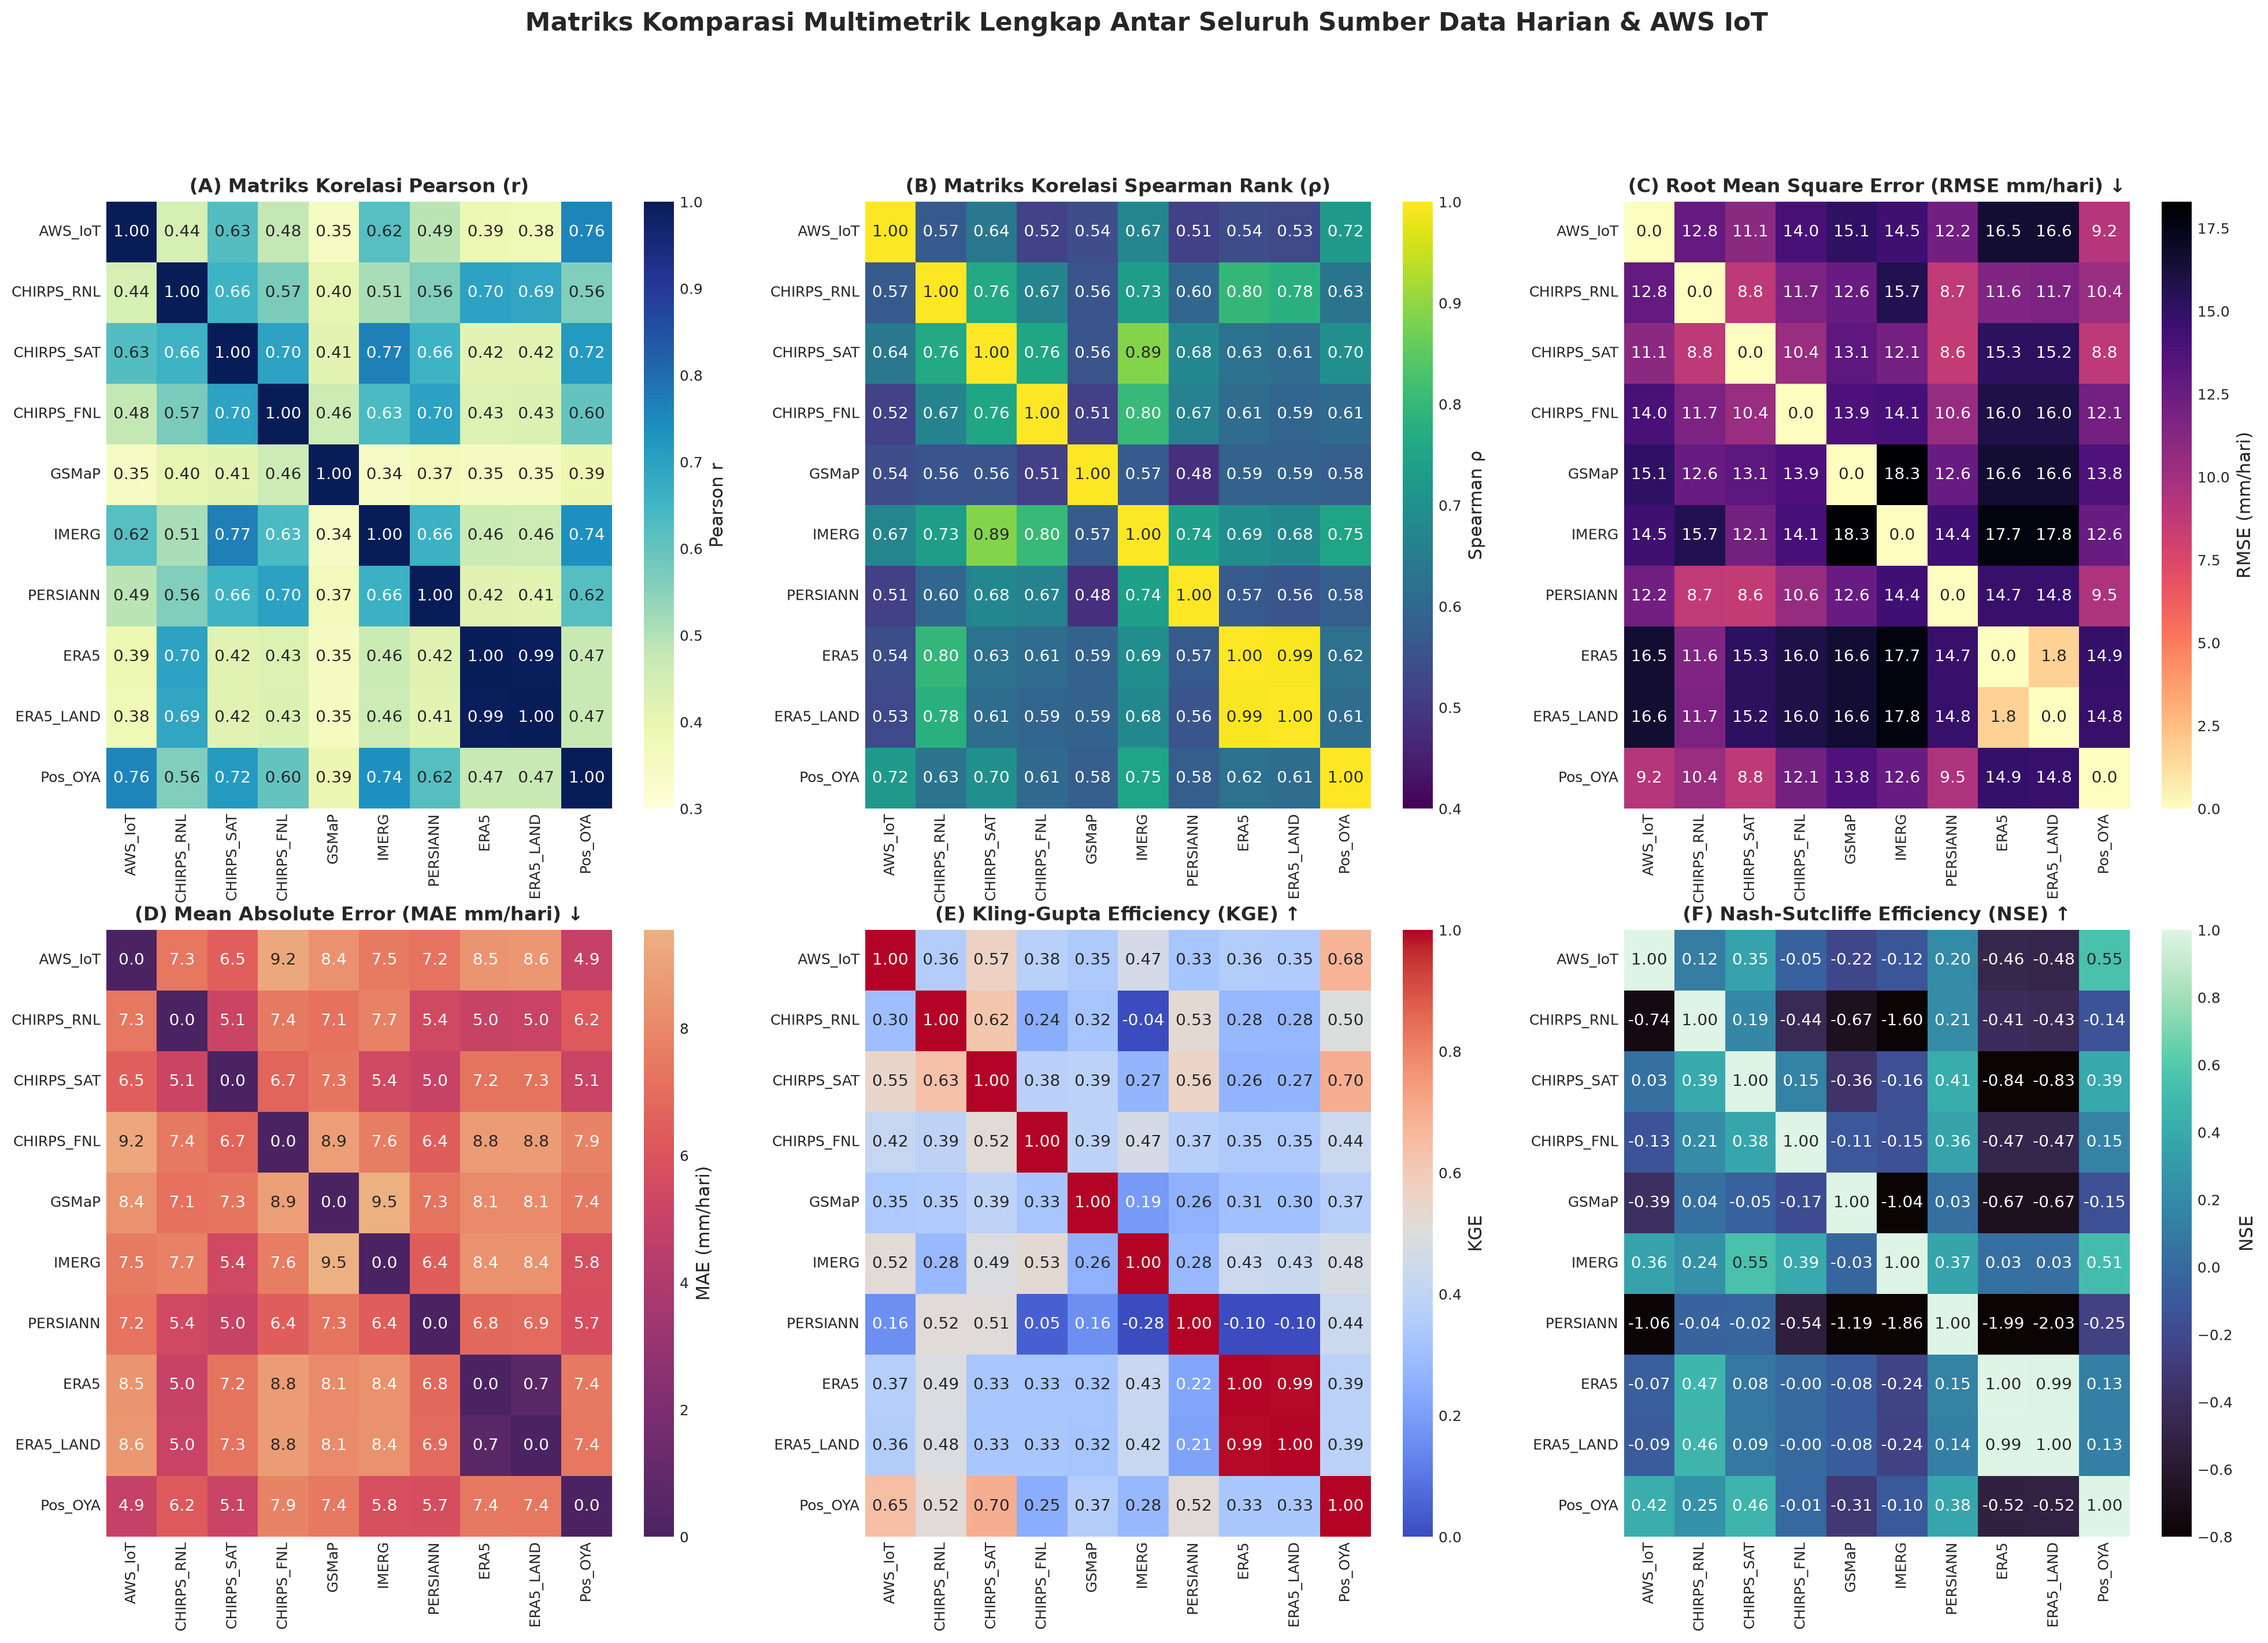
\includegraphics[width=0.98\textwidth]{09_heatmap_multimetrik_inter_model_harian.png}
    \caption{Matriks Heatmap Inter-Model $10 \times 10$ untuk 6 Metrik Kunci: (A) Pearson $r$, (B) Spearman $\rho$, (C) RMSE, (D) MAE, (E) KGE, dan (F) NSE.}
    \label{fig:multimetric_grid}
\end{figure}

\begin{figure}[htbp]
    \centering
    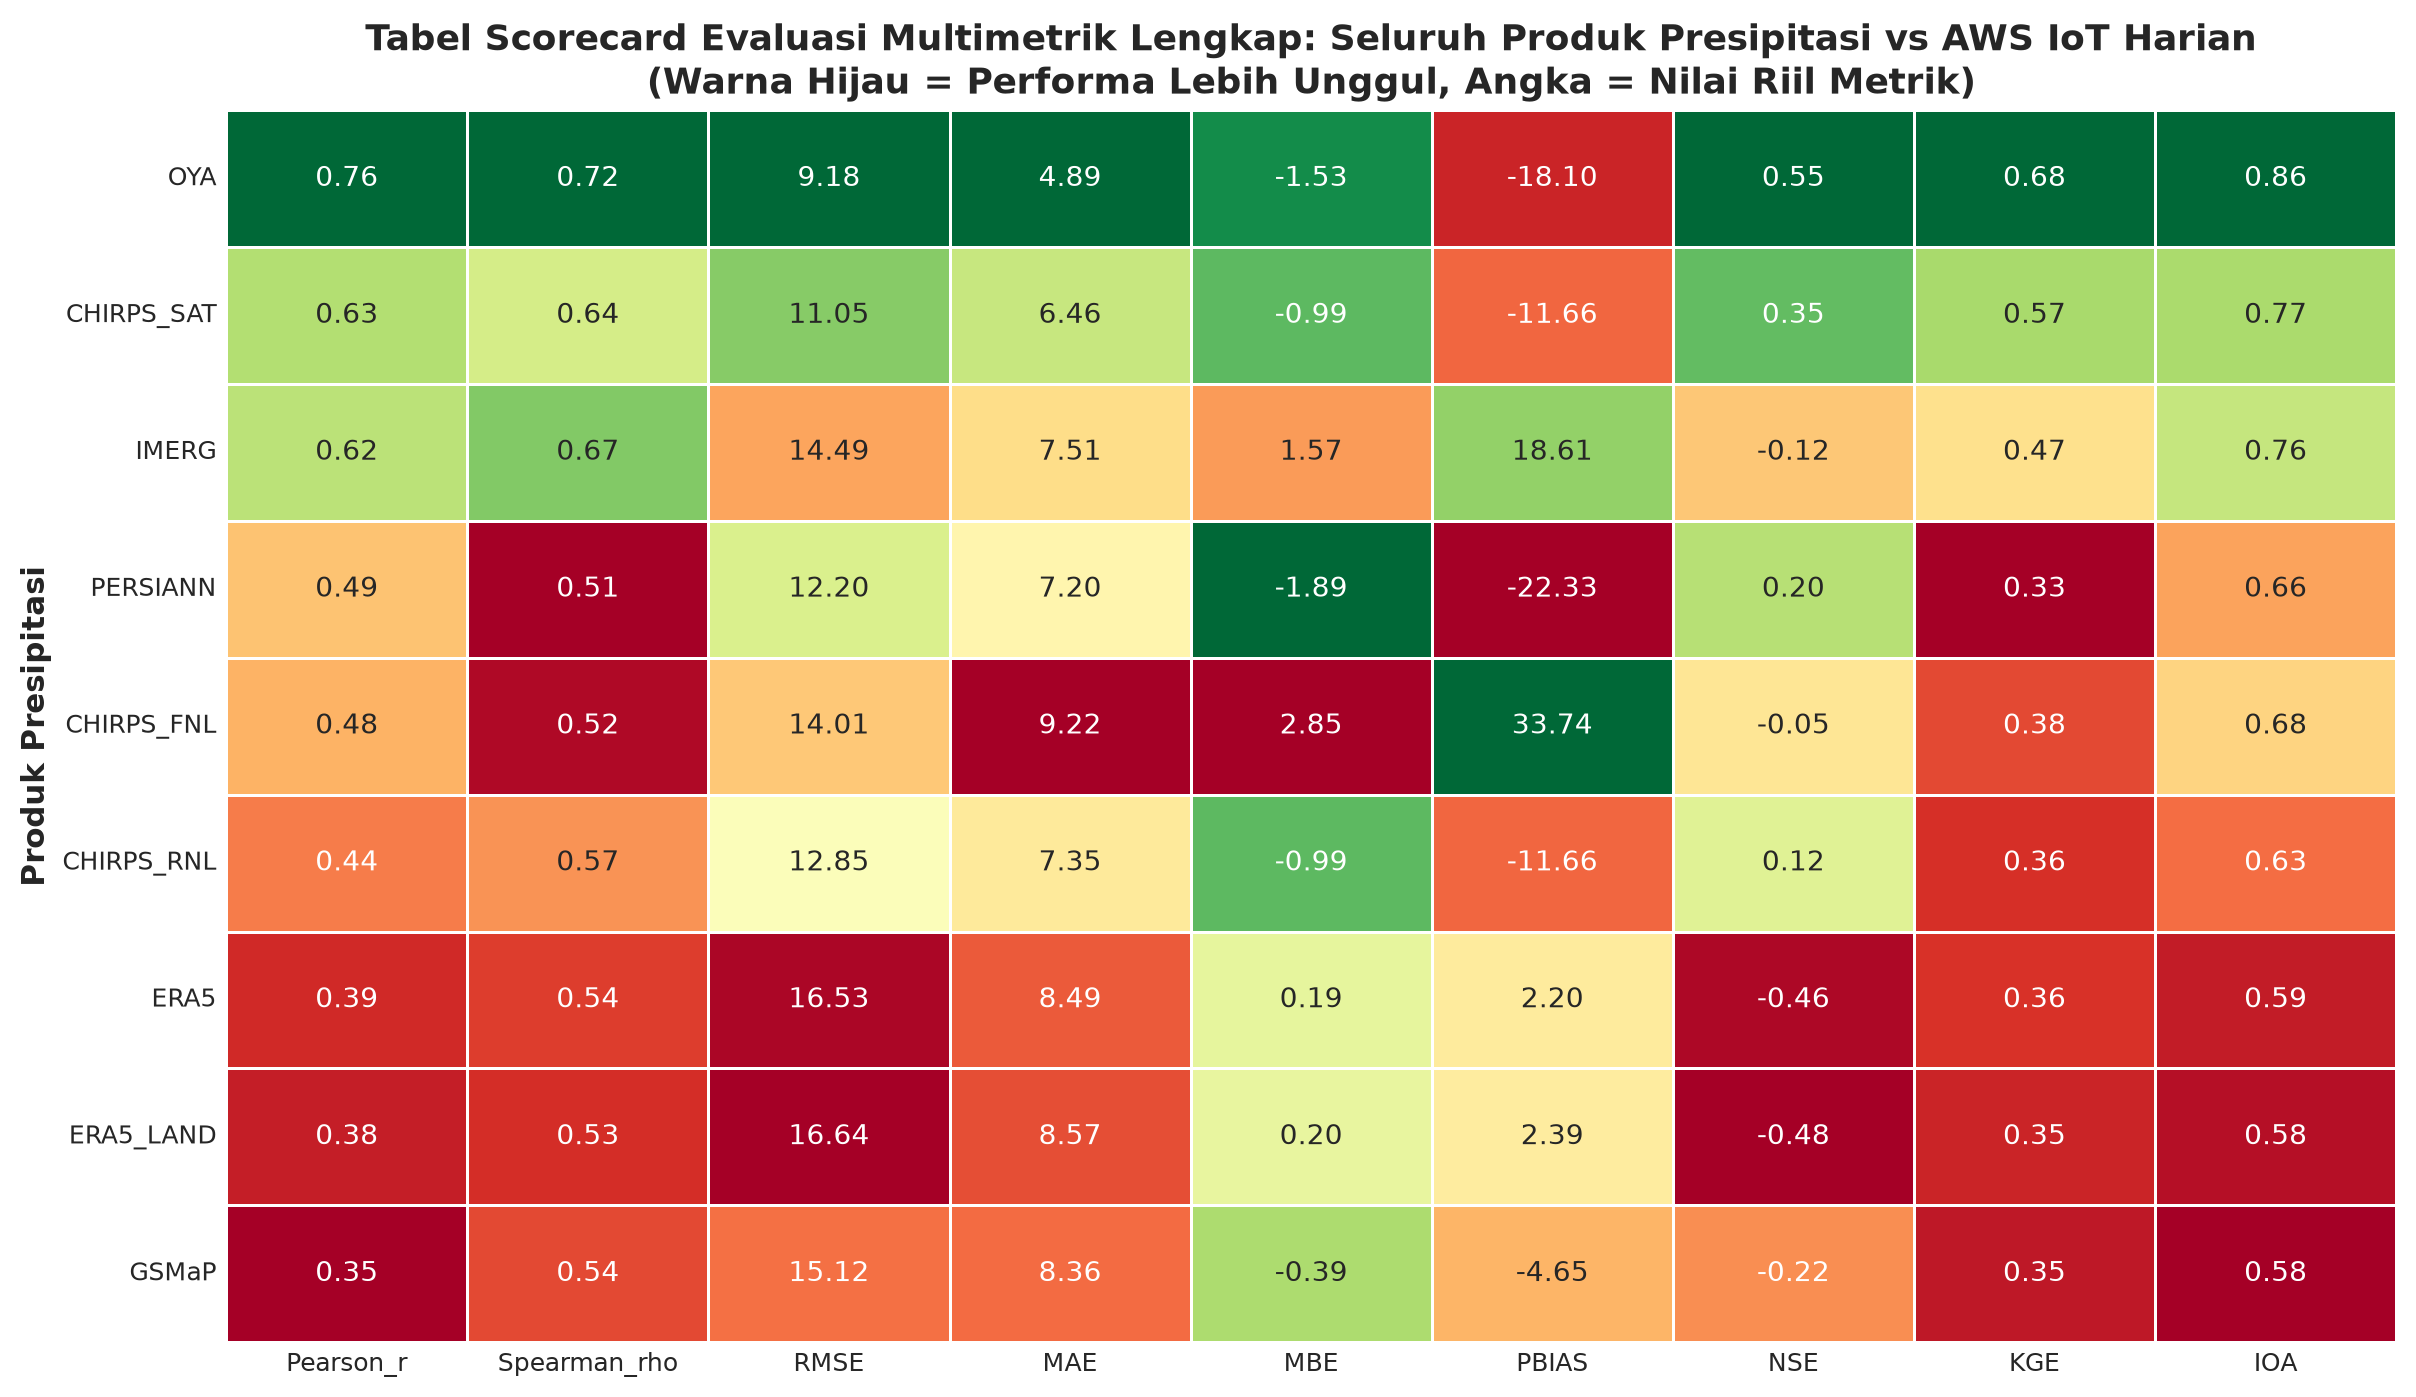
\includegraphics[width=0.95\textwidth]{10_heatmap_evaluasi_multimetrik_harian_vs_aws.png}
    \caption{Scorecard Evaluasi Multimetrik Lengkap: Nilai Riil Metrik dan Gradien Performa Seluruh Produk terhadap Stasiun AWS IoT Harian.}
    \label{fig:scorecard}
\end{figure}

\FloatBarrier

% =============================================================================
\section{Kesimpulan \& Rekomendasi Terapan}
% =============================================================================
Berdasarkan investigasi multi-skala hidrometeorologi di Kabupaten Kebumen, diperoleh kesimpulan fundamental sebagai berikut:

\begin{enumerate}[leftmargin=*]
    \item \textbf{Produk Satelit Harian Terbaik}: \texttt{NASA GPM IMERG} terbukti sebagai produk satelit dengan akurasi harian tertinggi ($r = 0{,}619, \rho = 0{,}672, \text{MAE} = 7{,}51\text{ mm/hari}, \text{IOA} = 0{,}759$), disusul oleh \texttt{CHIRPS\_SAT} ($r = 0{,}625, \text{KGE} = 0{,}569$) dan \texttt{JAXA GSMaP} ($r = 0{,}350, \rho = 0{,}543$).
    \item \textbf{Fenomena Lonjakan Akurasi Multi-Temporal}: Agregasi dari skala 1-jam ke 24-jam terbukti efektif mereduksi derau fluktuasi sub-harian dan pergeseran spasial awan konvektif, menghasilkan peningkatan korelasi rata-rata $+49{,}5\%$ hingga $+266{,}7\%$.
    \item \textbf{Termodinamika Diurnal Tropis}: Dinamika hujan lokal di Stasiun Jerukagung Kebumen didominasi oleh hujan konvektif sore hari (pukul 15:00--18:00 WIB), yang dipicu oleh akumulasi radiasi surya maksimum pada siang hari (12:00--13:00 WIB) dan didukung oleh penurunan tekanan semidiurnal atmosfer.
    \item \textbf{Standar Lookback Sequence Model LSTM}: Berdasarkan analisis ACF/PACF, panjang jendela sekuens untuk arsitektur deep learning presipitasi distandarisasi pada $\text{LOOKBACK} = 24$ jam (resolusi 1-jam) untuk menangkap siklus diurnal penuh, $\text{LOOKBACK} = 120$ (resolusi 1-menit) dengan fitur siklik, serta $\text{LOOKBACK} = 7$--$14$ hari (resolusi harian) untuk menangkap gelombang sinoptik mingguan tanpa risiko \textit{vanishing gradient} dan pemborosan VRAM GPU.
\end{enumerate}

\end{document}
